
\documentclass{article}
%\usepackage{figure}
\usepackage{graphicx}
\usepackage{float}
\usepackage{setspace}

\usepackage[a4paper, left=.4in, right=.4in, top=1in, bottom=1.2in]{geometry}
\begin{document}
\doublespacing
\section{\(\xi_a= 1/15000\), and \(\xi_w=1/600\)}\label{sec:sec1}

\begin{itemize}
    \item$\xi_p= 1000$:
        \begin{figure}[H]
            \centering
            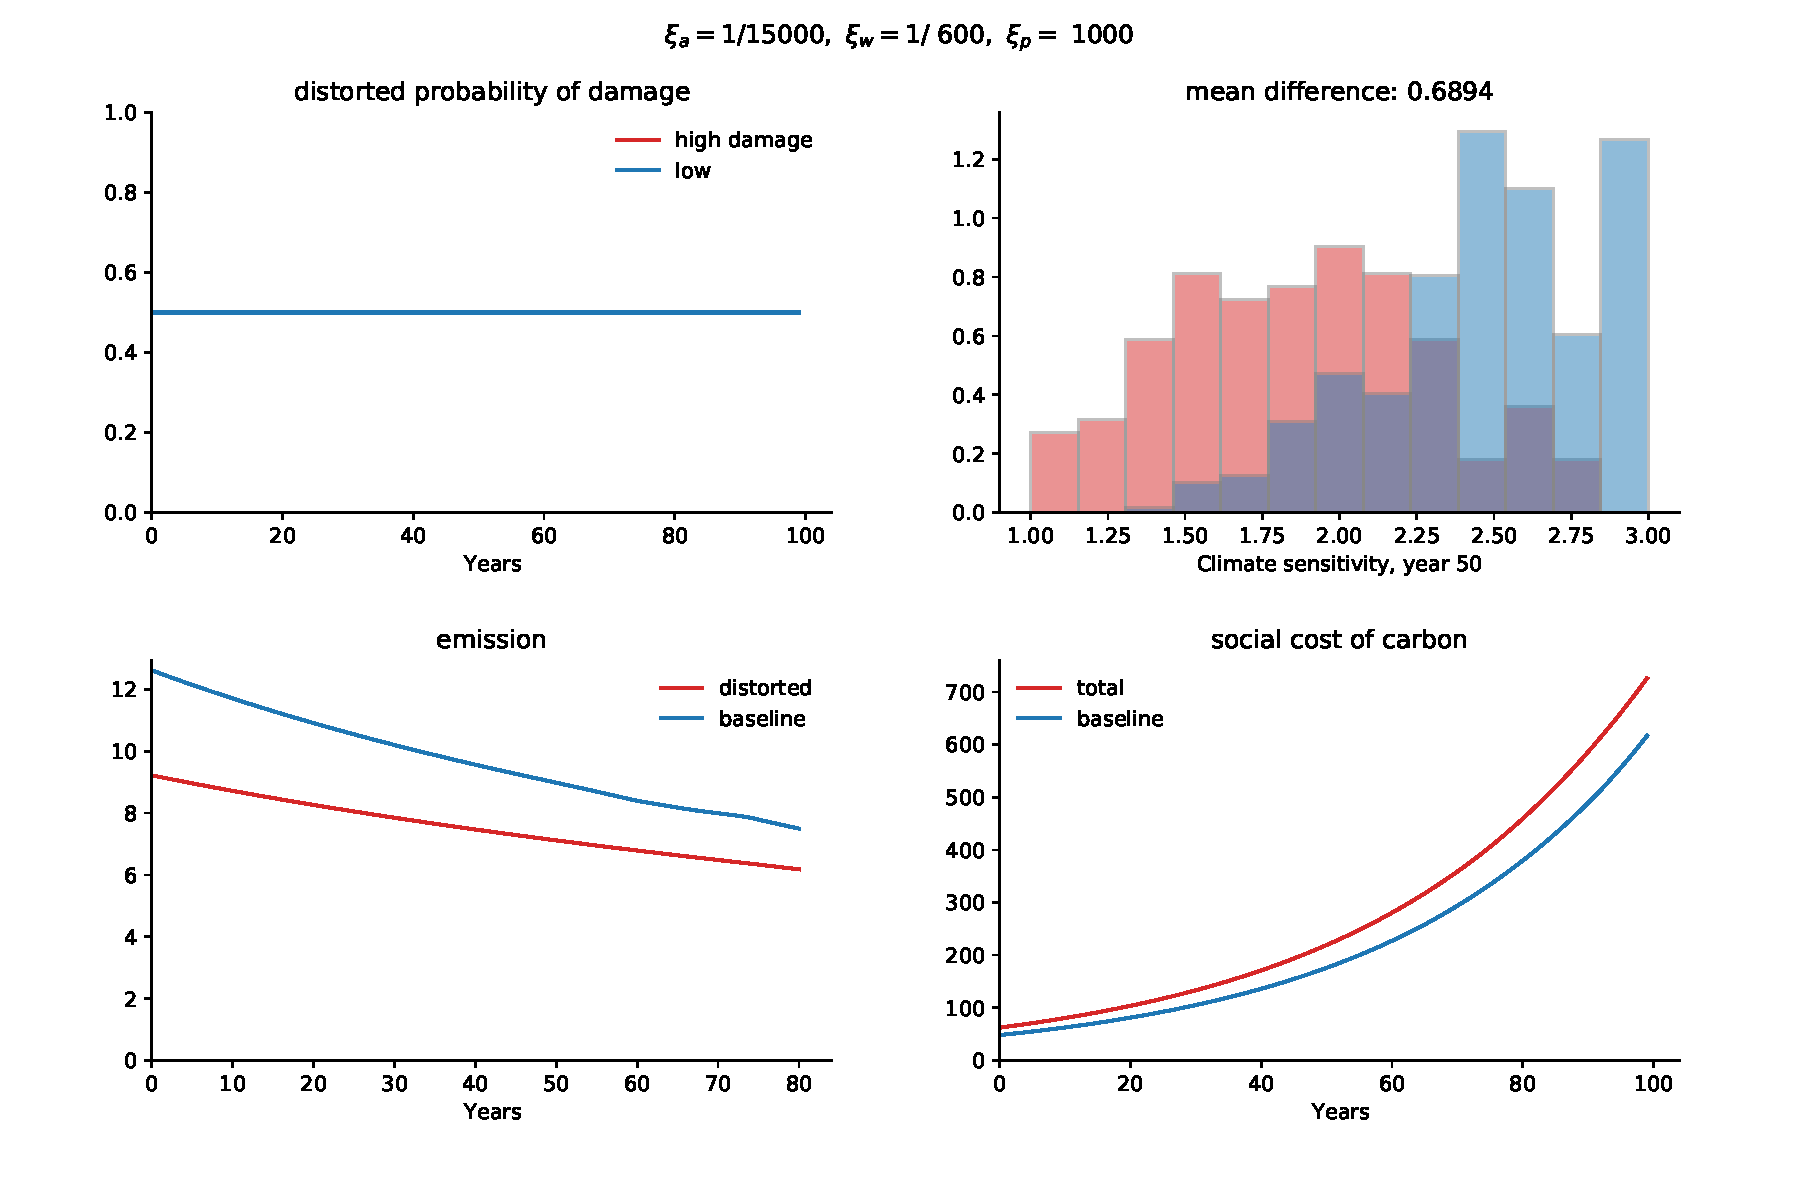
\includegraphics[width=\linewidth]{notebook/15_600_1000.pdf}
            \caption{$\xi_p= 1000$}
            \label{fig:notebook/15_600_1000}
        \end{figure}
        \newpage
    \item$\xi_p= 60\xi_w$:
        \begin{figure}[H]
            \centering
            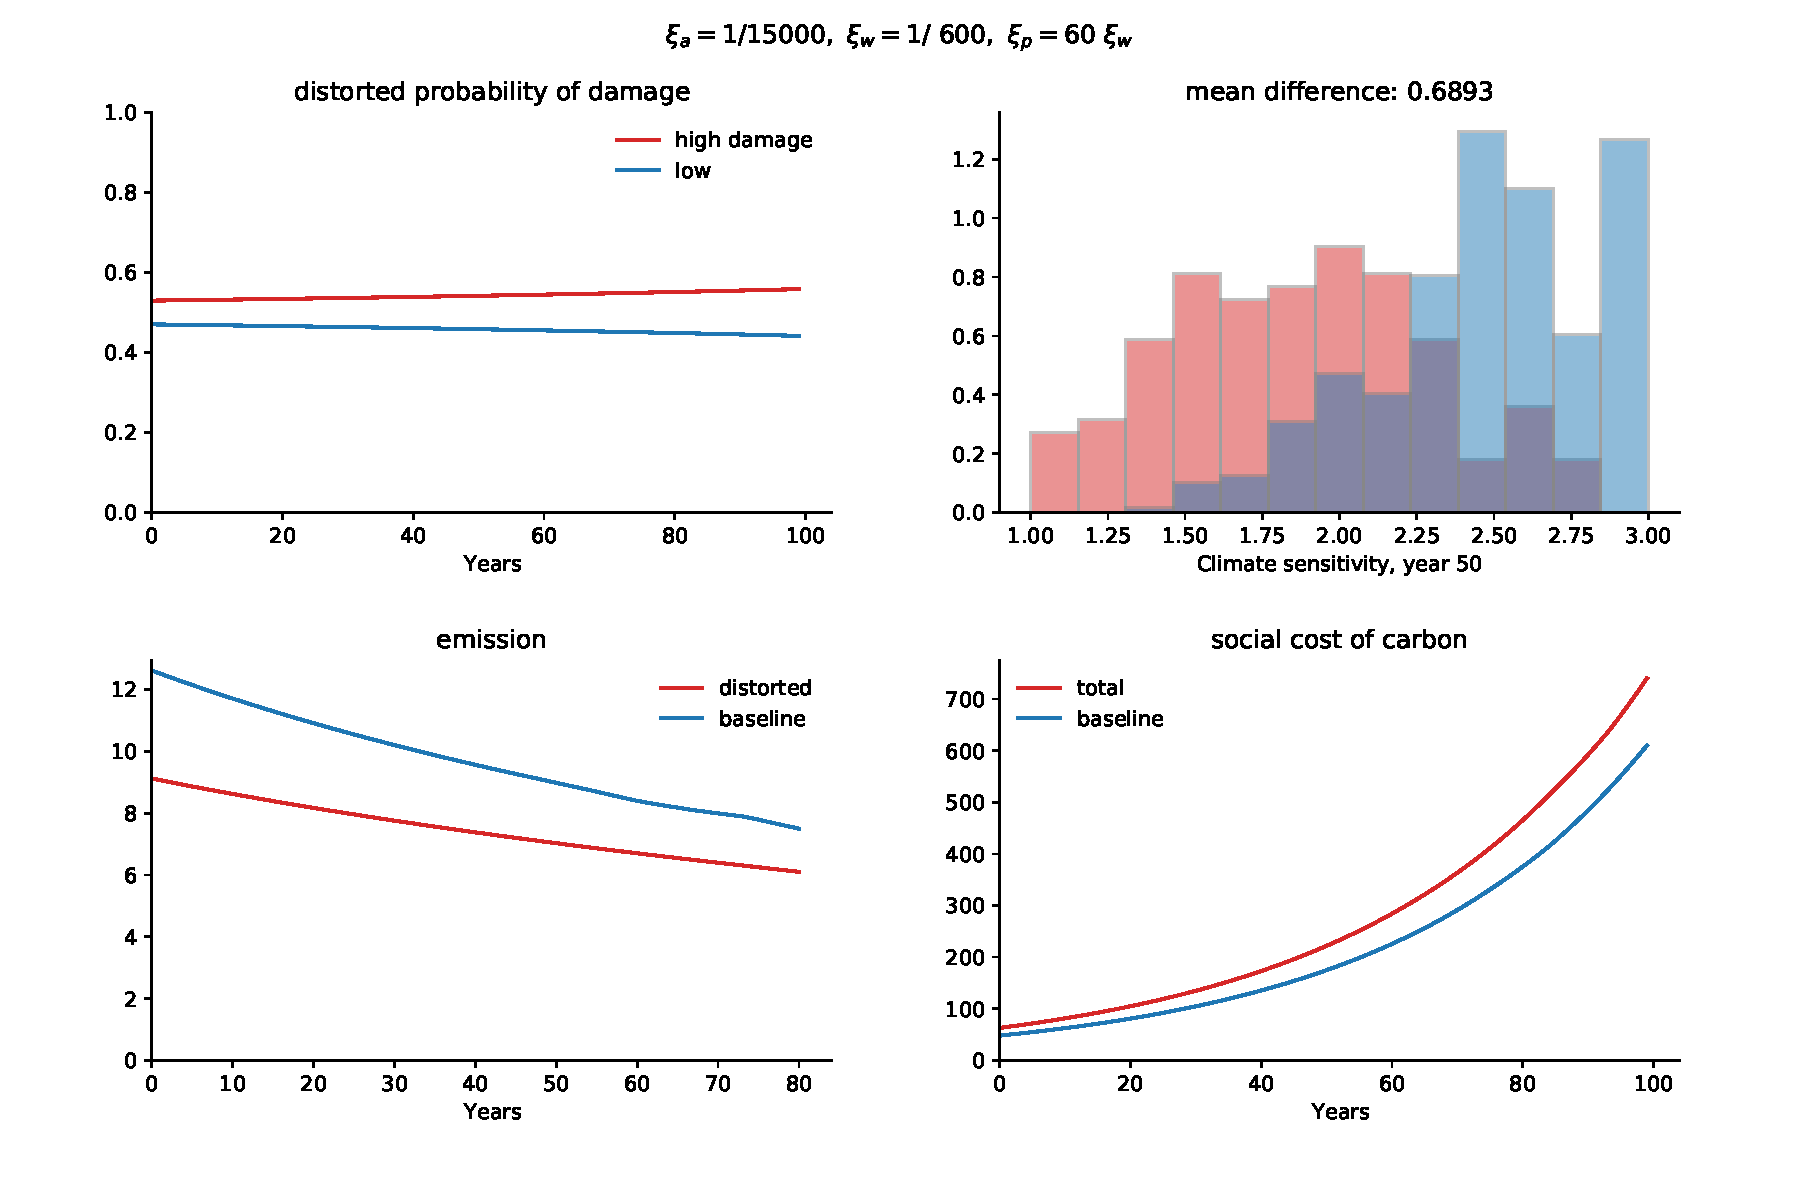
\includegraphics[width=\linewidth]{notebook/15_600_60.pdf}
            \caption{$\xi_p=60\xi_w$}
            \label{fig:notebook/phi_n}
        \end{figure}
        \newpage
\item $\xi_p=30\xi_w$
    \begin{figure}[H]
        \centering
        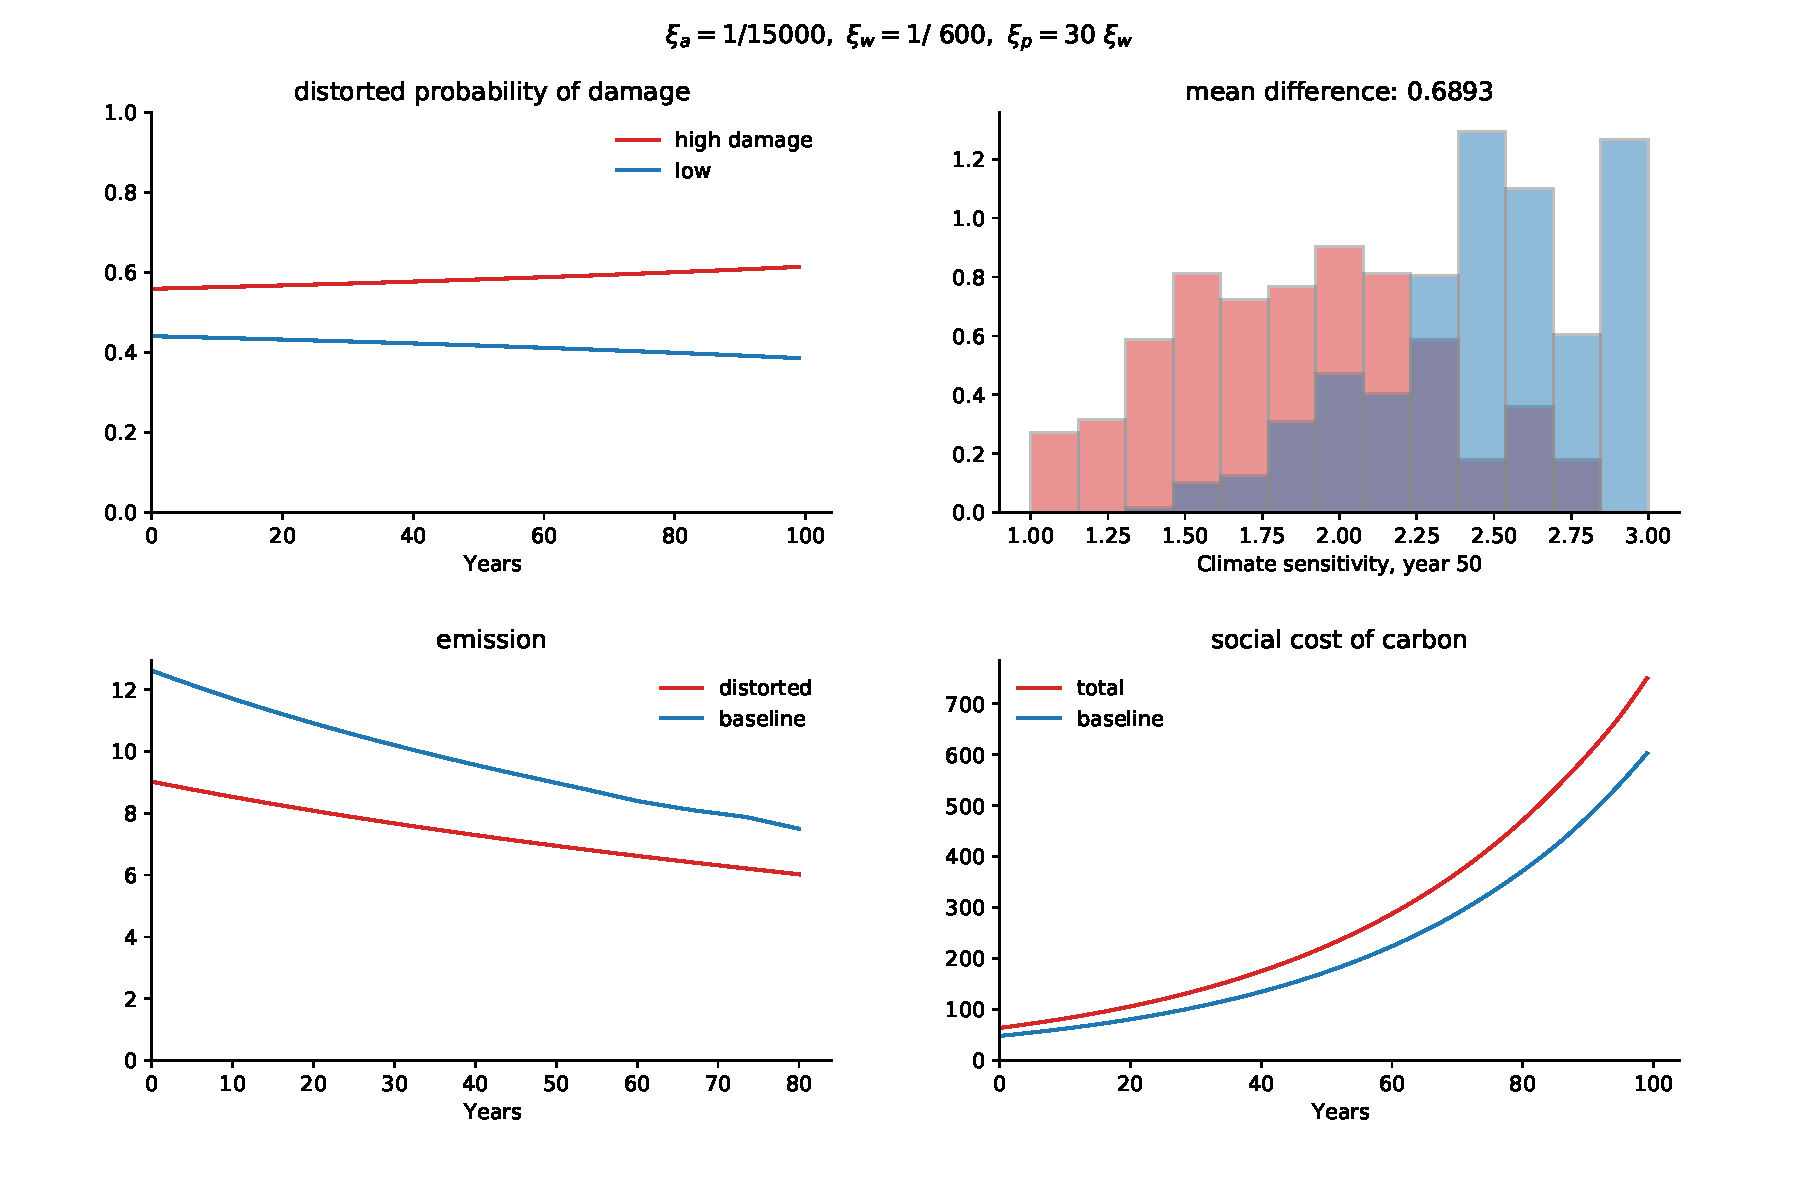
\includegraphics[width=\linewidth]{notebook/15_600_30.pdf}
        \caption{$\xi_p= 30\xi_w$}
        \label{fig:notebook/phi_x10}
    \end{figure}
    \newpage
\item$\xi_p= \xi_w$:
       \begin{figure}[H]
           \centering
           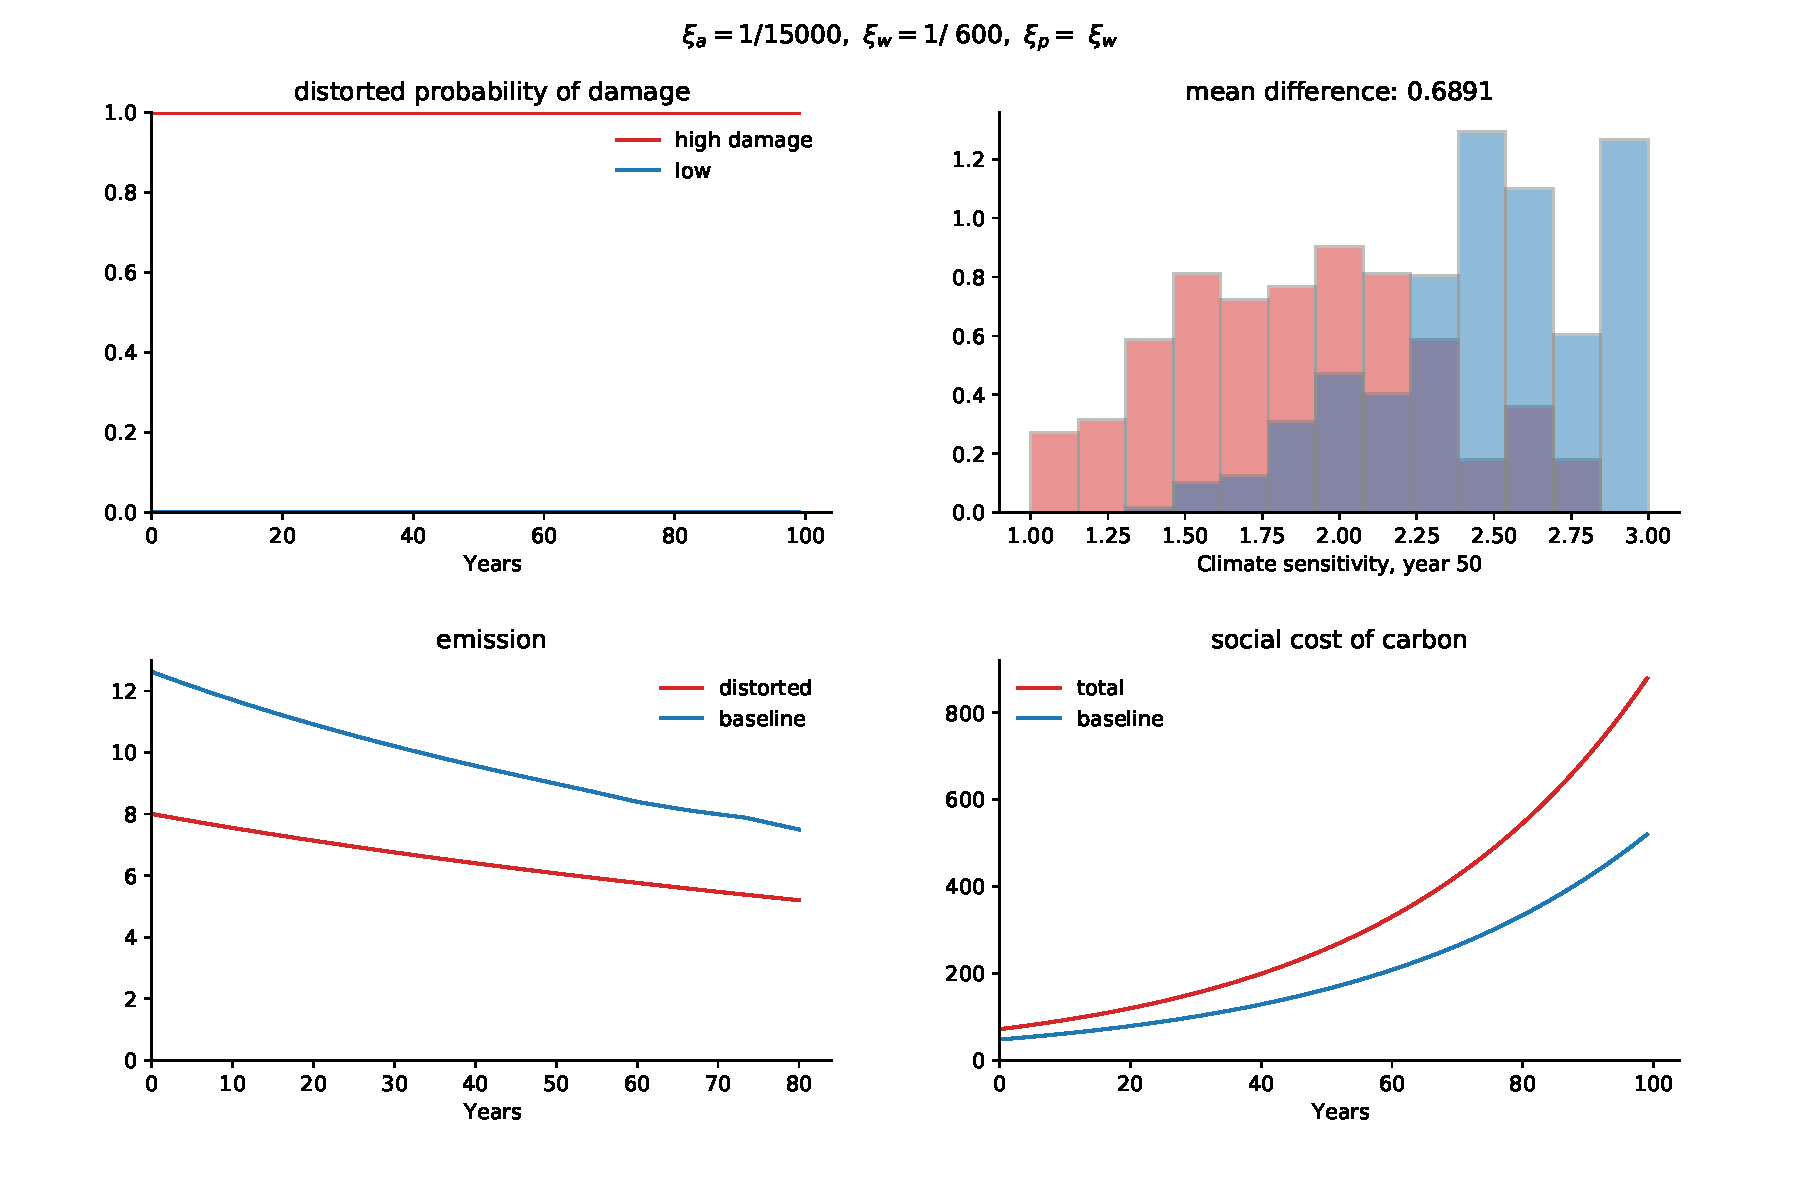
\includegraphics[width=\linewidth]{notebook/15_600_1.pdf}
           \caption{$\xi_p= \xi_w$}
           \label{fig:notebook/phi_x5}
       \end{figure}
       \newpage
\end{itemize}

\section{\(\xi_a= 1/15000\) and \(\xi_w=1/900\)}\label{sec:sec2}
\begin{itemize}
    \item \(\xi_p= 1000\):
        \begin{figure}[H]
            \centering
            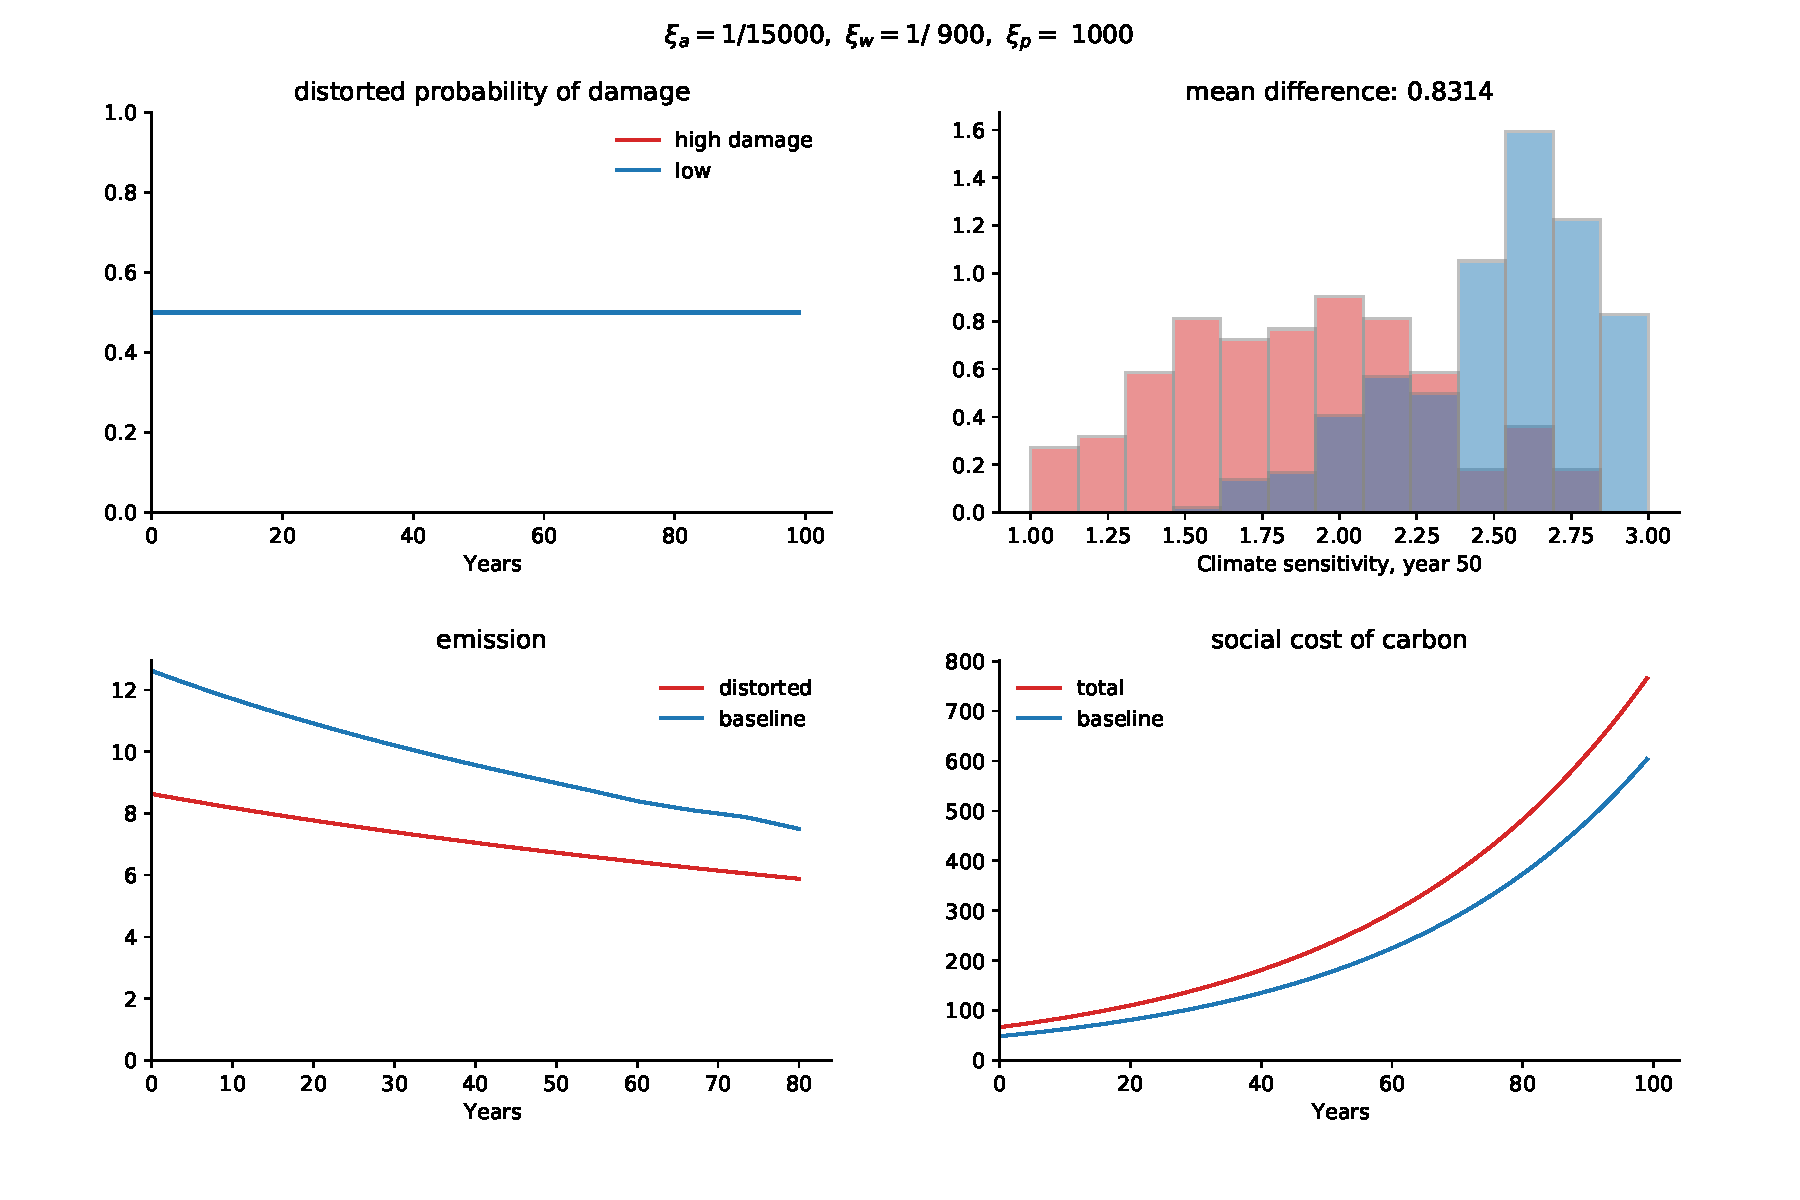
\includegraphics[width=\linewidth]{notebook/15_900_1000.pdf}
            \caption{\(\xi_p=1000\)}
            \label{fig:notebook/15_900_90}
        \end{figure}
        \newpage
    \item \(\xi_p= 90\xi_w\)
        \begin{figure}[H]
            \centering
            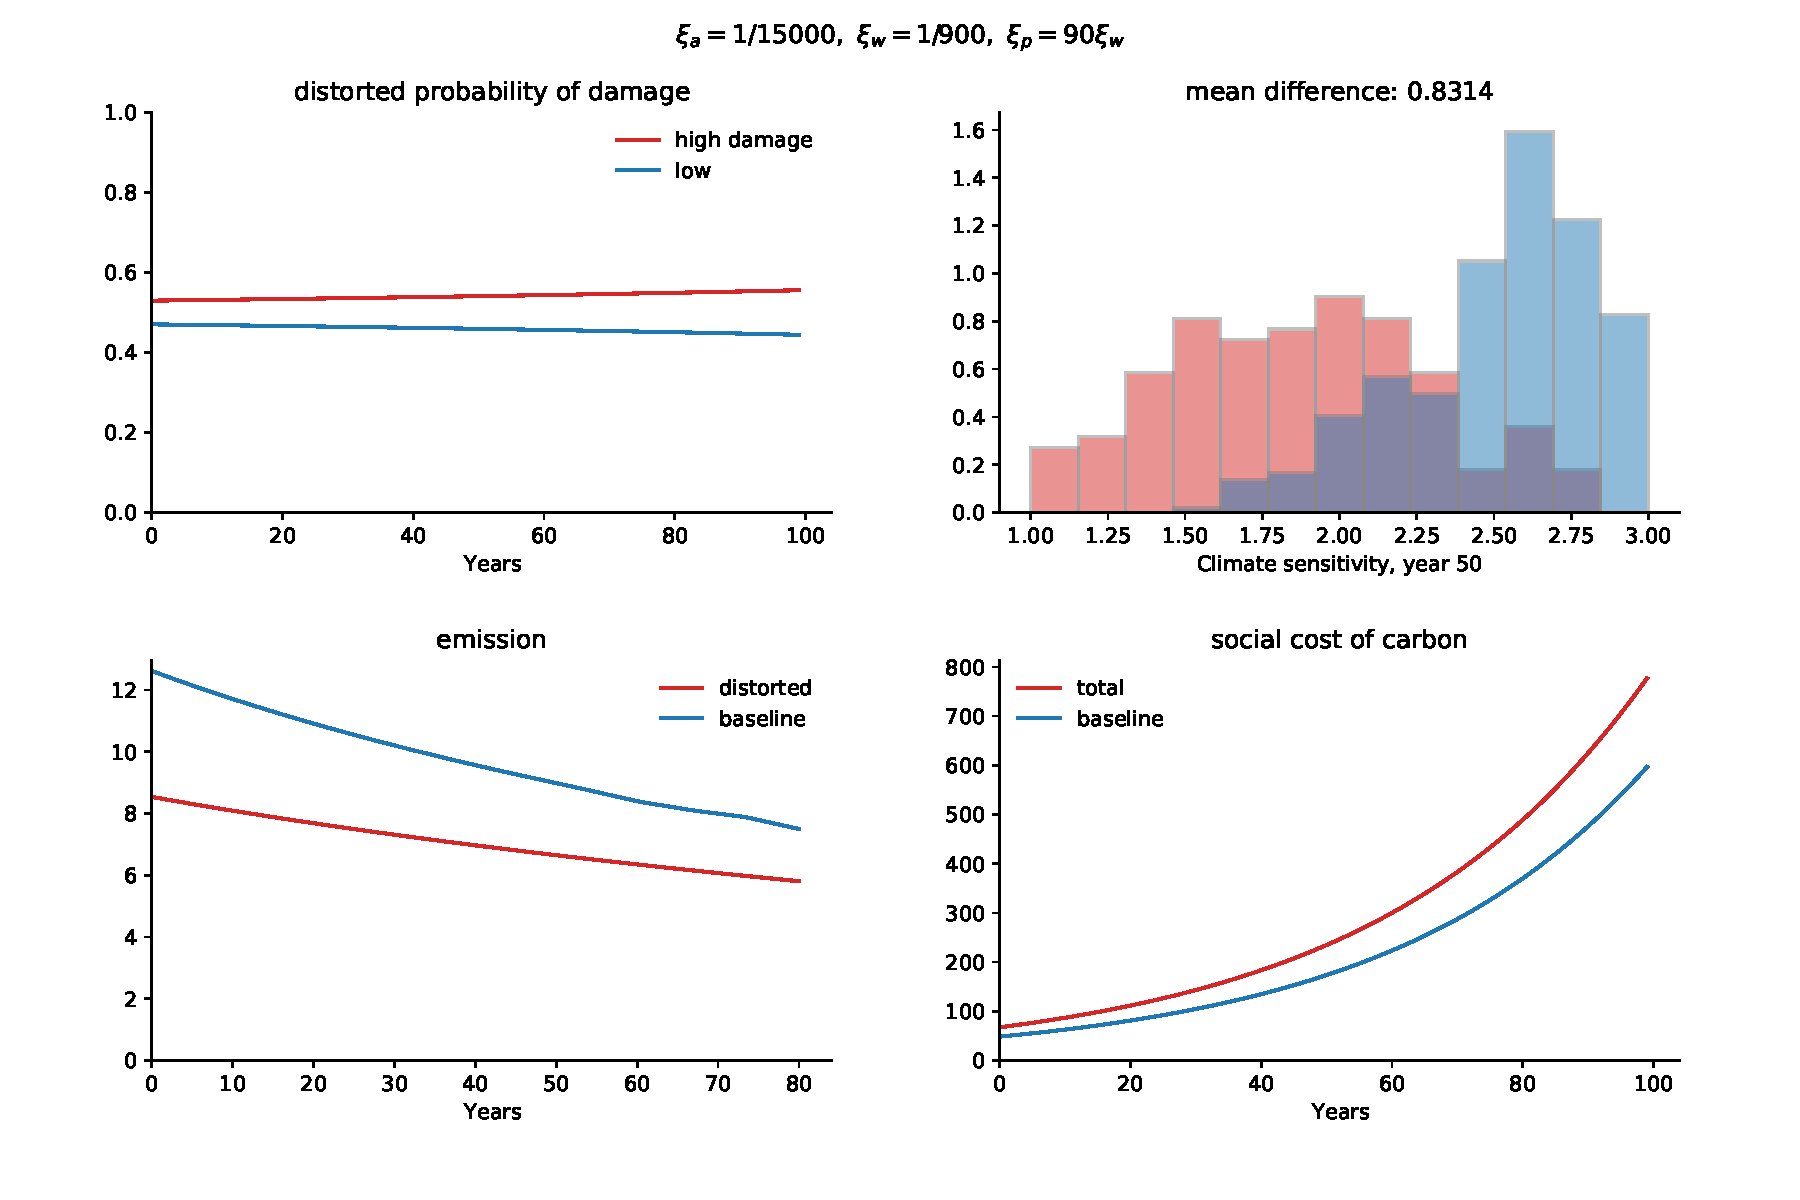
\includegraphics[width=\linewidth]{notebook/15_900_90.pdf}
            \caption{\(\xi_p=90\xi_w\)}
            \label{fig:notebook/15_900_90}
        \end{figure}
        \newpage
    \item \(\xi_p=45\xi_w\)
        \begin{figure}[H]
            \centering
            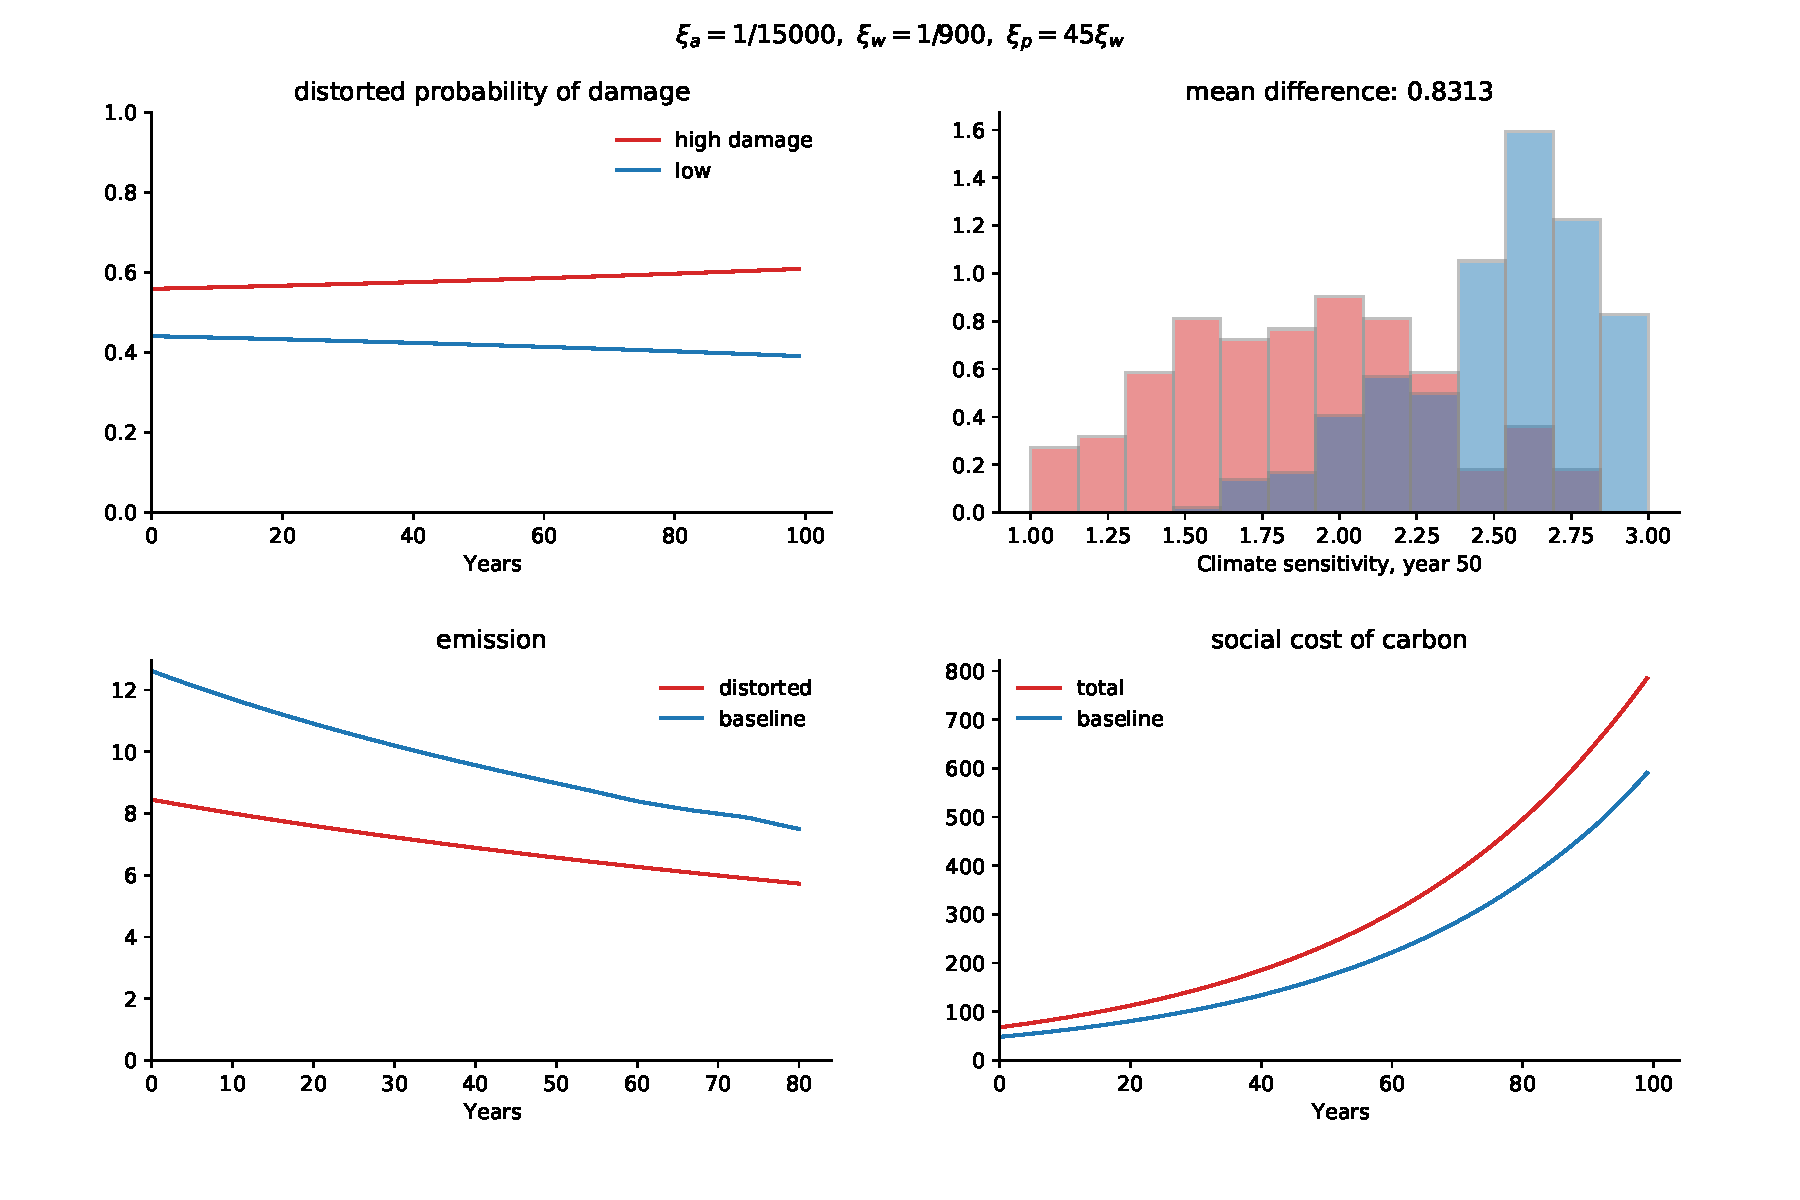
\includegraphics[width=\linewidth]{notebook/15_900_45.pdf}
            \caption{\(\xi_p=45\xi_w\)}
            \label{fig:notebook/15_900_45}
        \end{figure}
        \newpage
    \item \(\xi_p=\xi_w\)
        \begin{figure}[H]
            \centering
            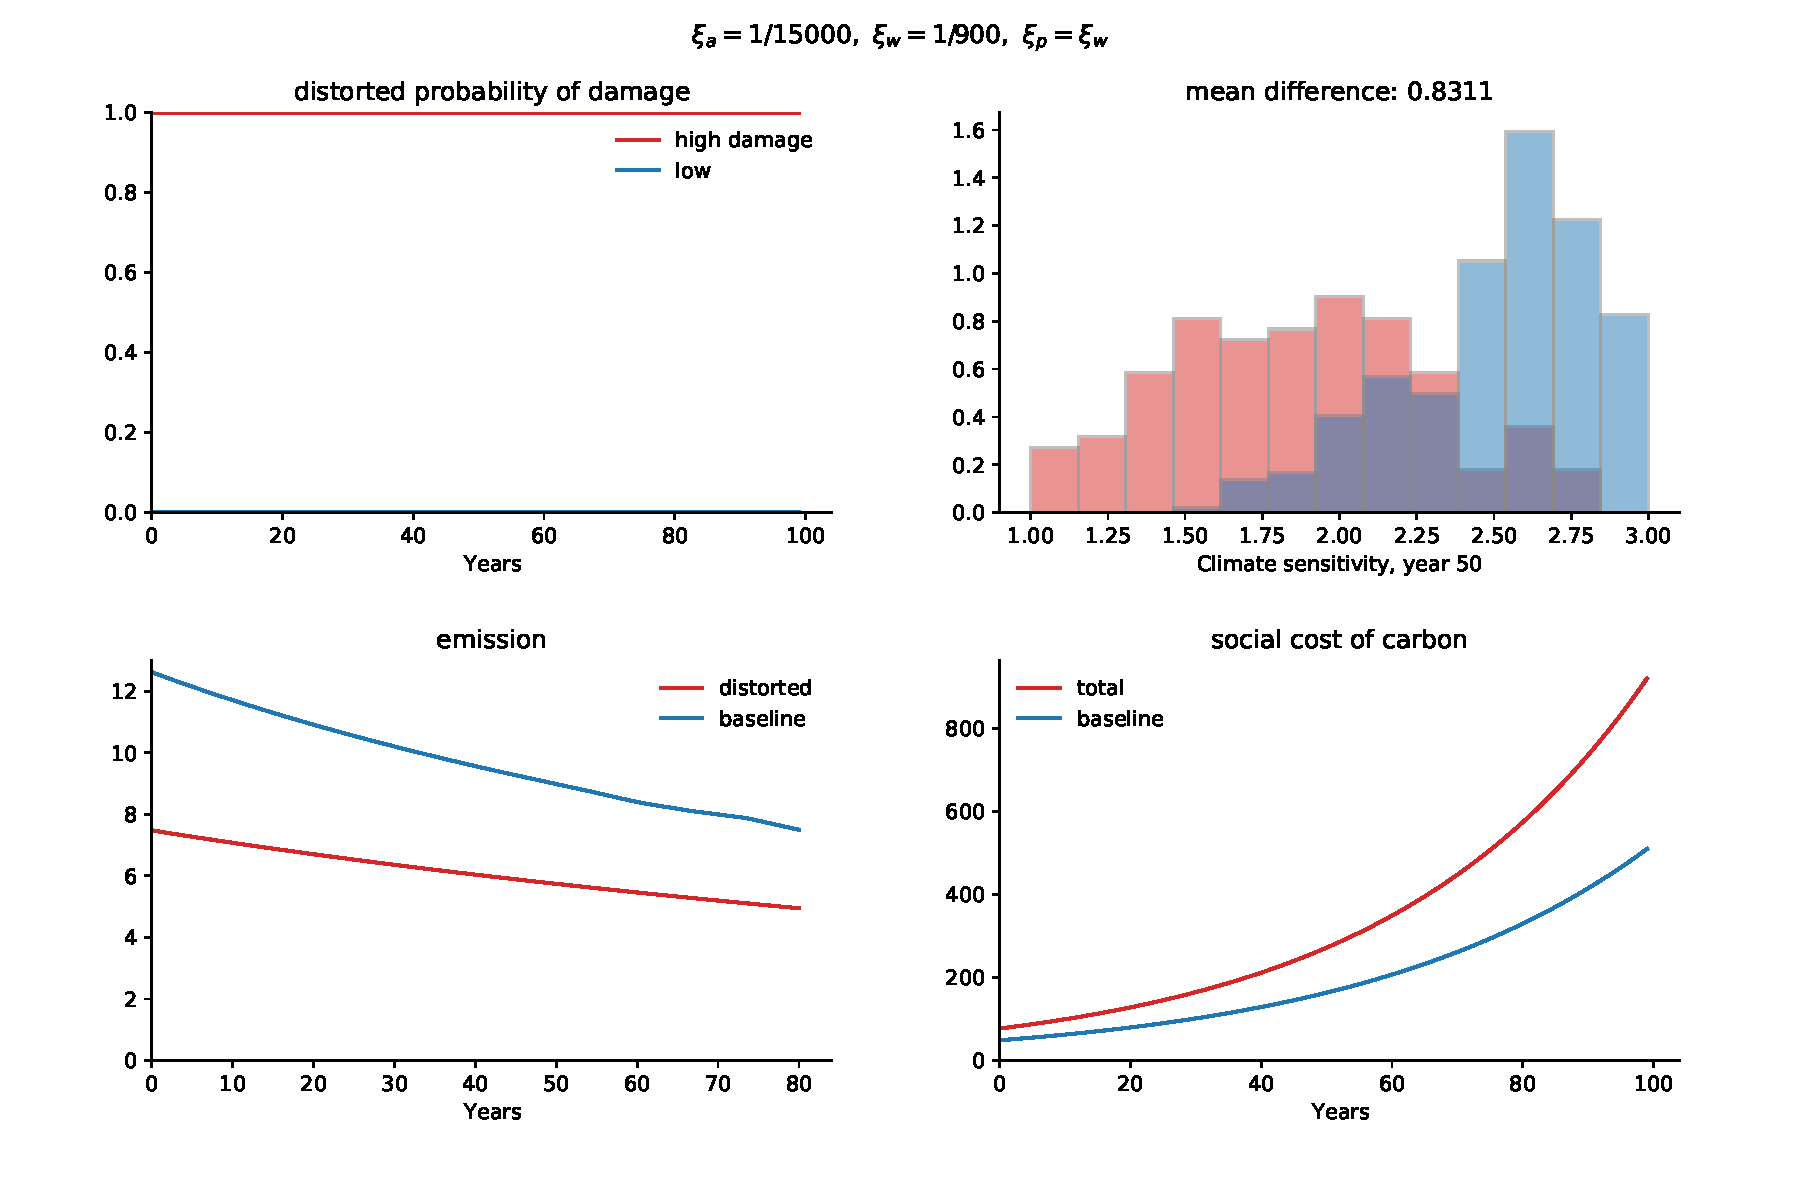
\includegraphics[width=\linewidth]{notebook/15_900_1.pdf}
            \caption{\(\xi_p=\xi_w\)}
            \label{fig:notebook/15_900_45}
        \end{figure}
\end{itemize}
\newpage
\section{\(\xi_a= 1/10000\), and \(\xi_w=1/600\)}\label{sec:sec3}

\begin{itemize}
    \item$\xi_p= 1000$:
        \begin{figure}[H]
            \centering
            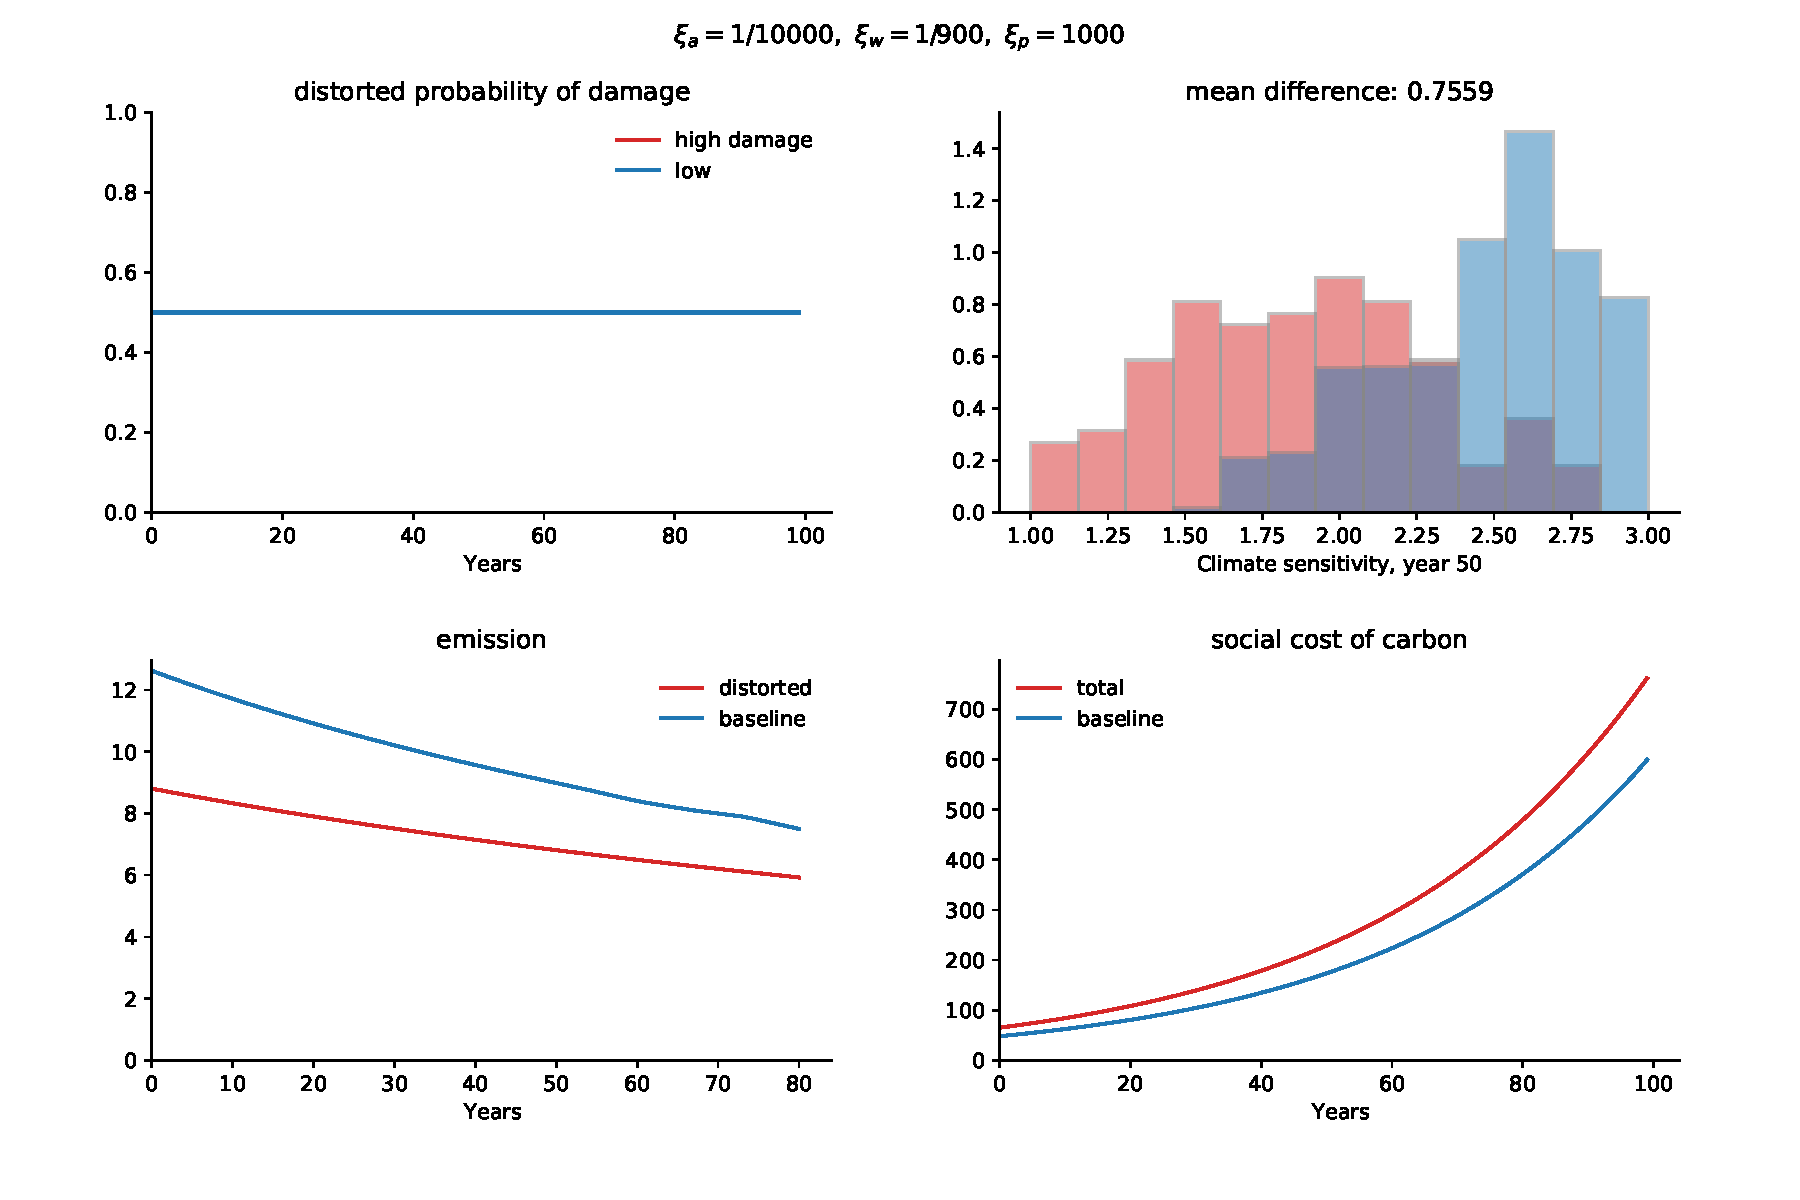
\includegraphics[width=\linewidth]{notebook/10_600_1000.pdf}
            \caption{$\xi_p= 1000$}
            \label{fig:notebook/10_600_1000}
        \end{figure}
        \newpage
    \item$\xi_p= 60\xi_w$:
        \begin{figure}[H]
            \centering
            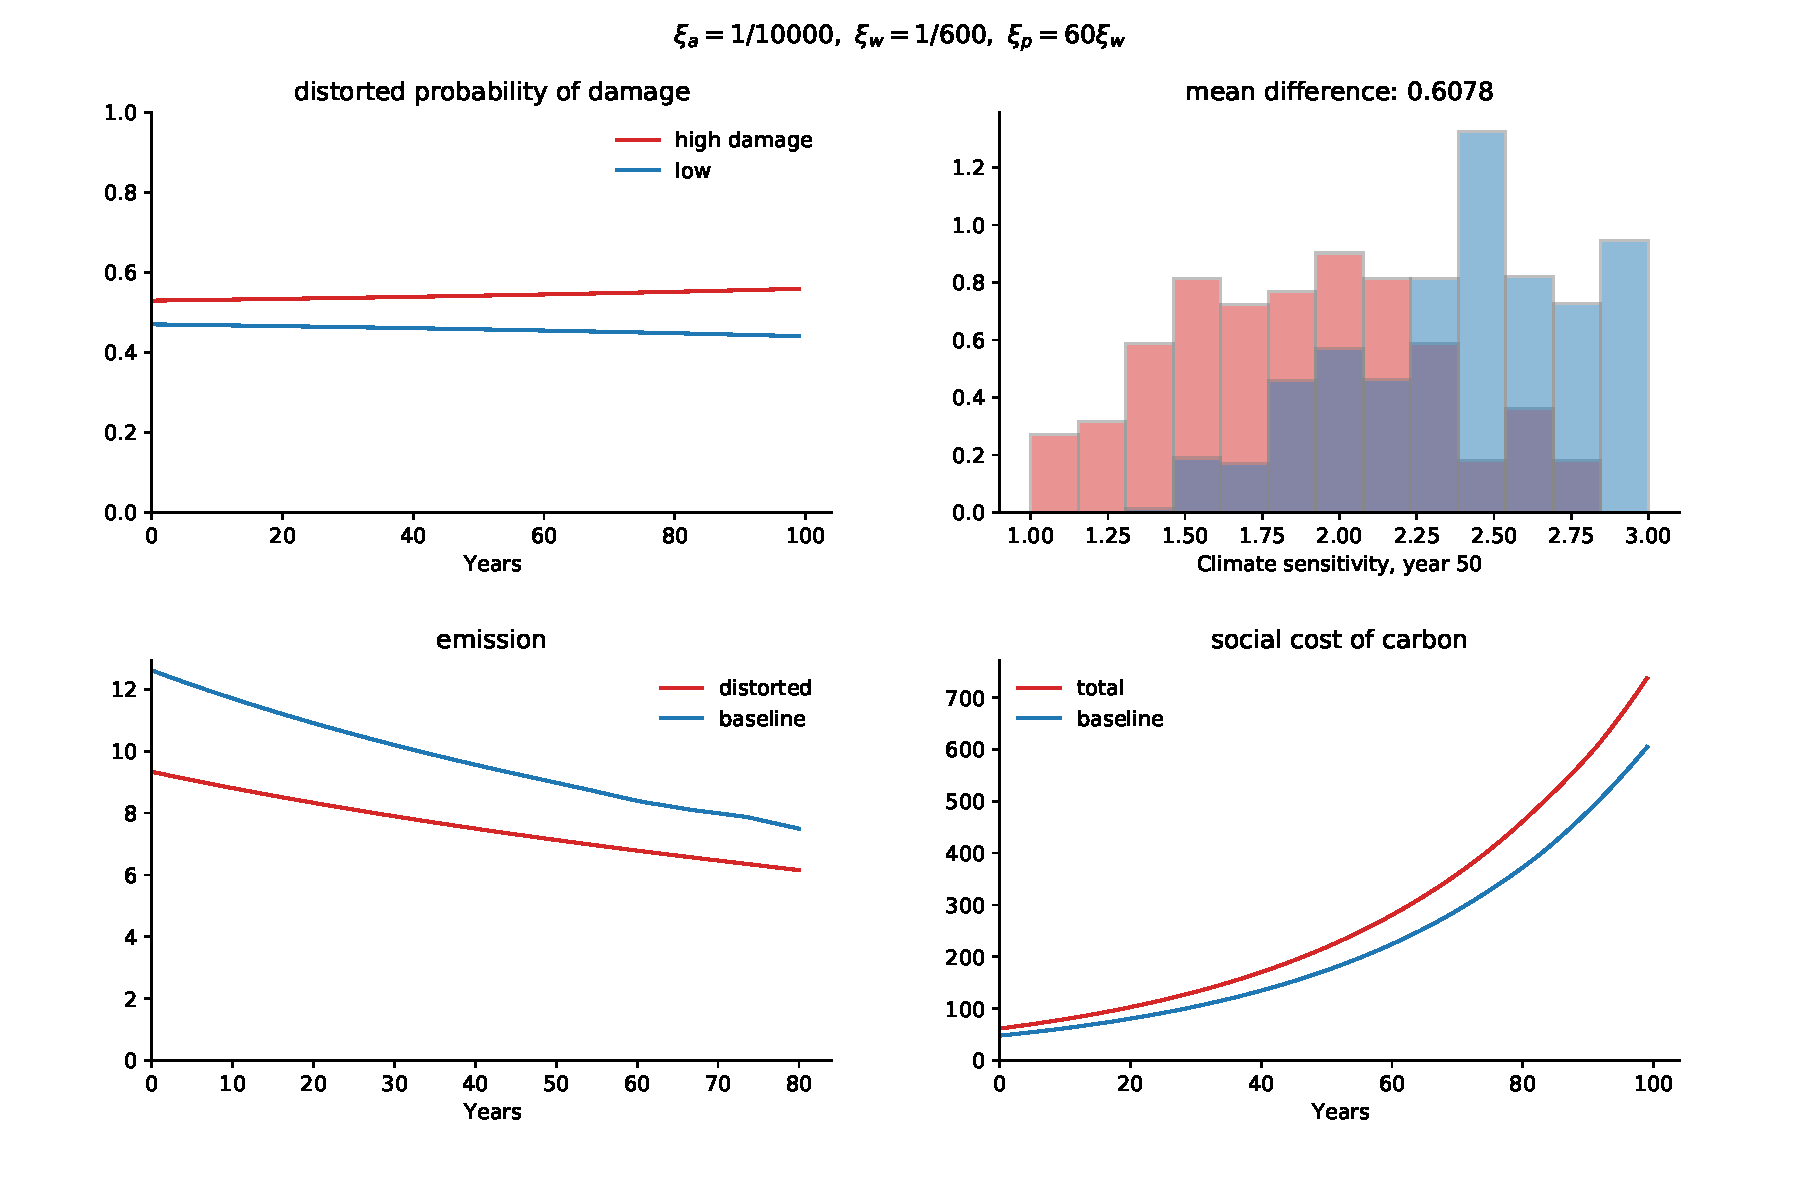
\includegraphics[width=\linewidth]{notebook/10_600_60.pdf}
            \caption{$\xi_p=60\xi_w$}
            \label{fig:notebook/10_600_60}  
        \end{figure}
        \newpage
\item $\xi_p=30\xi_w$
    \begin{figure}[H]
        \centering
        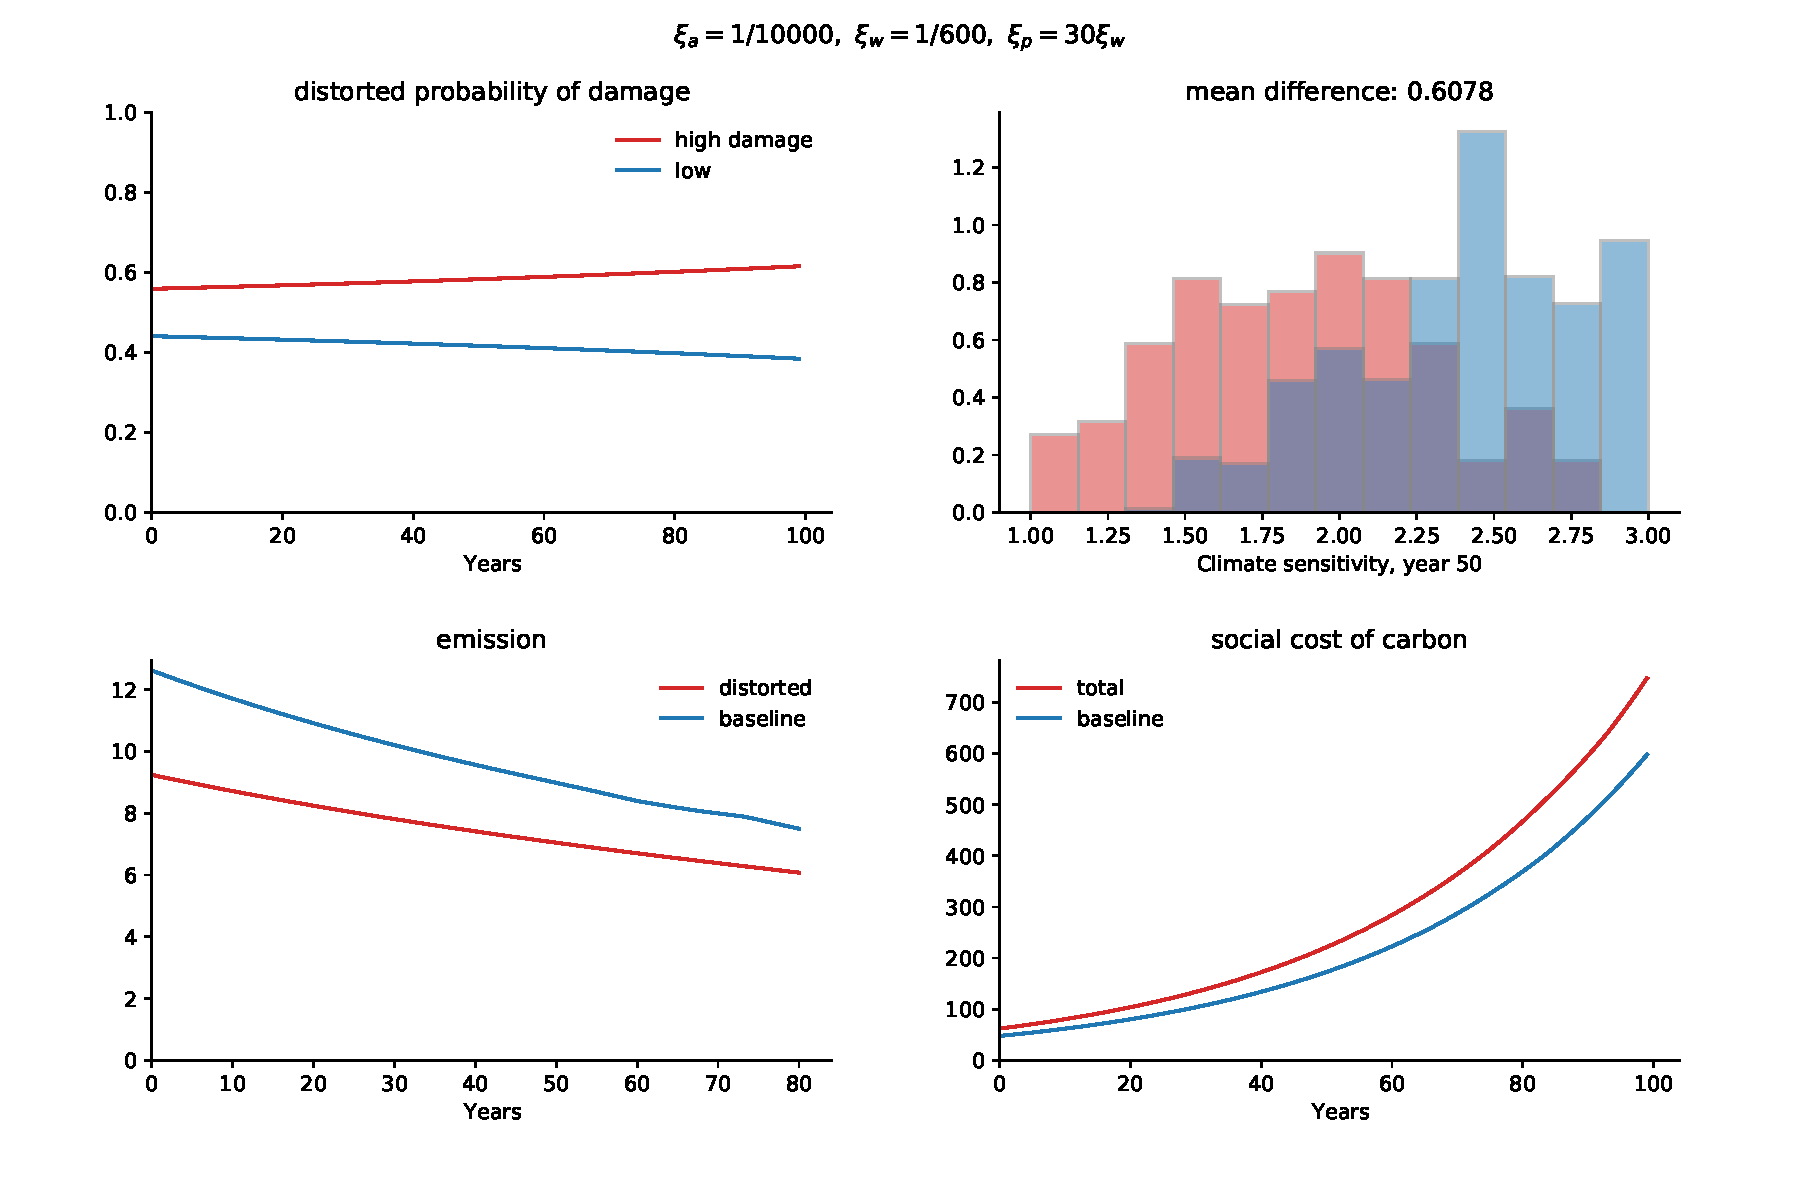
\includegraphics[width=\linewidth]{notebook/10_600_30.pdf}
        \caption{$\xi_p= 30\xi_w$}
        \label{fig:notebook/10_600_30}
    \end{figure}
    \newpage
\item$\xi_p= \xi_w$:
       \begin{figure}[H]
           \centering
           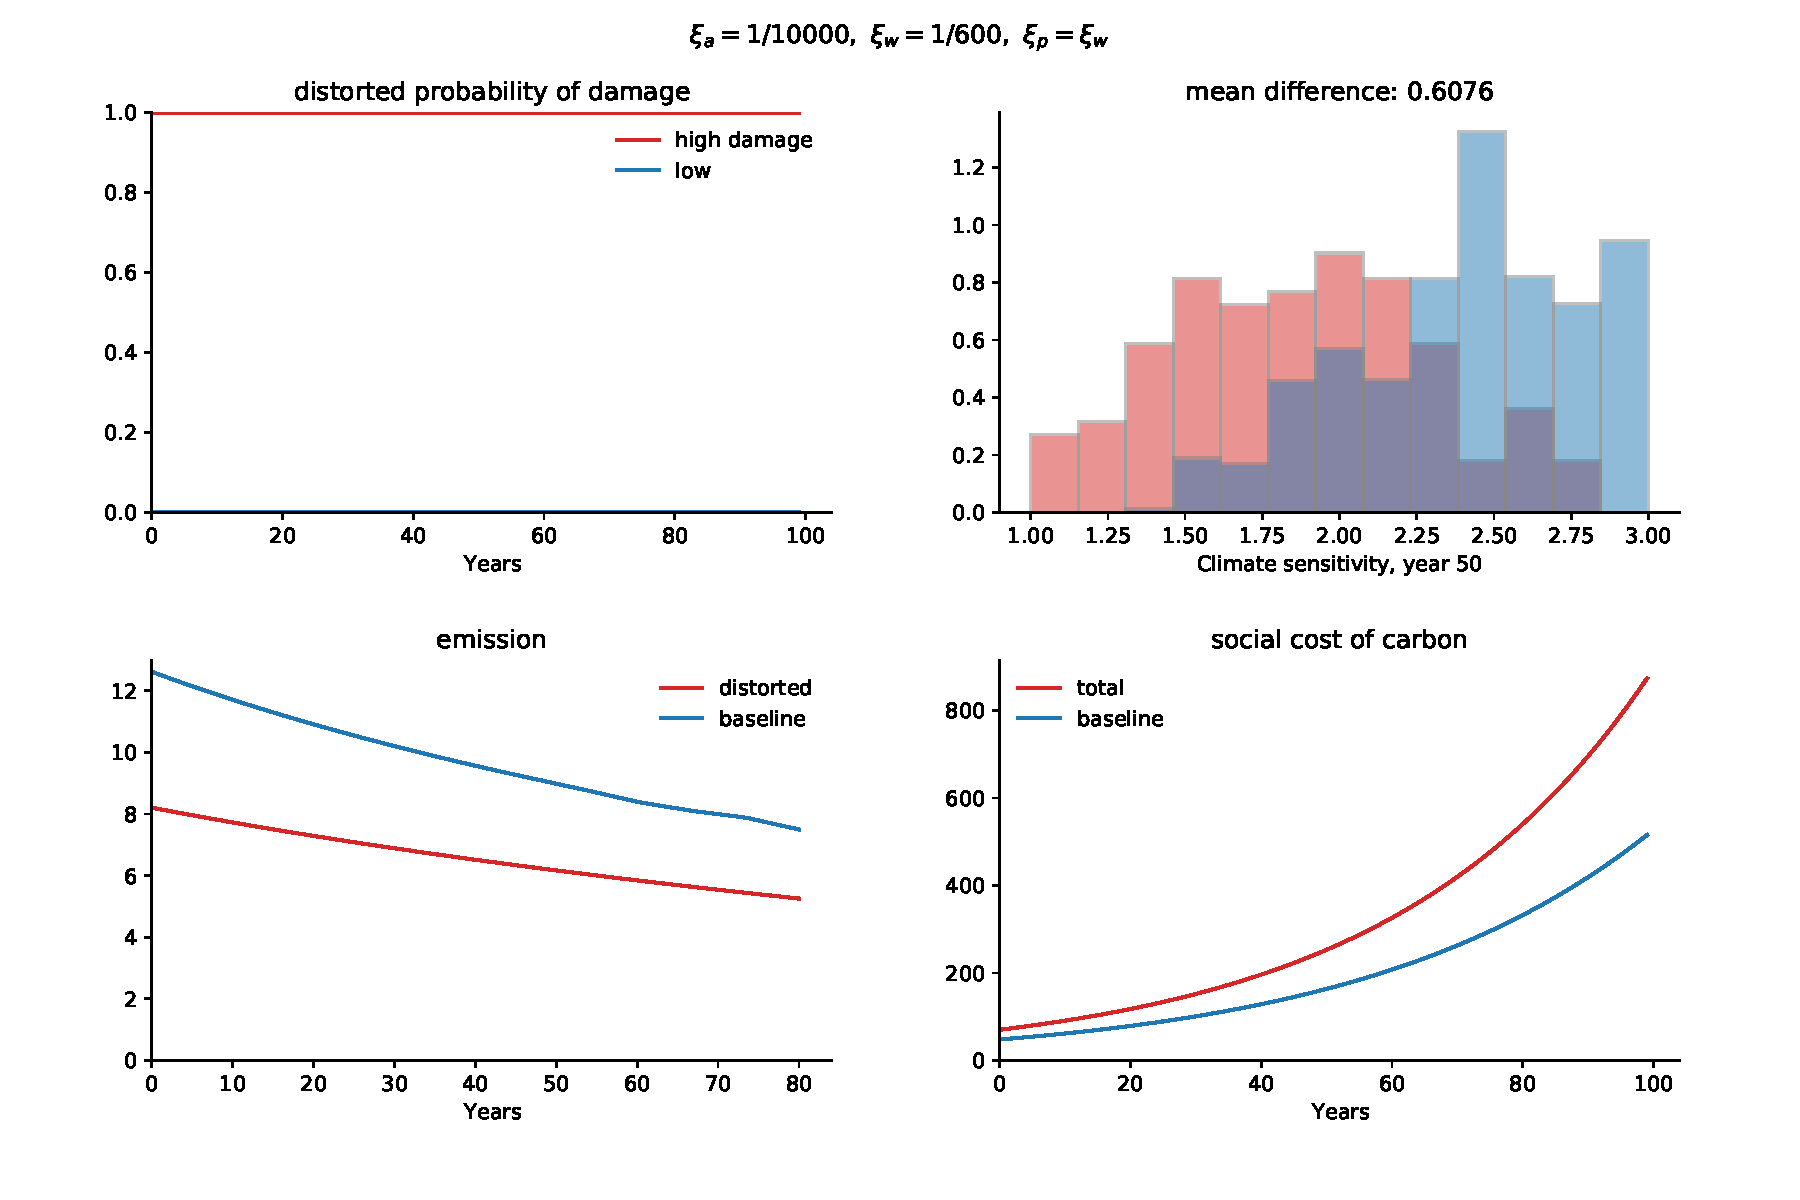
\includegraphics[width=\linewidth]{notebook/10_600_1.pdf}
           \caption{$\xi_p= \xi_w$}
           \label{fig:notebook/10_600_1}
       \end{figure}
\end{itemize}

\newpage
\section{\(\xi_a= 1/10000\) and \(\xi_w=1/900\)}\label{sec:sec4}
\begin{itemize}
    \item \(\xi_p= 1000\):
        \begin{figure}[H]
            \centering
            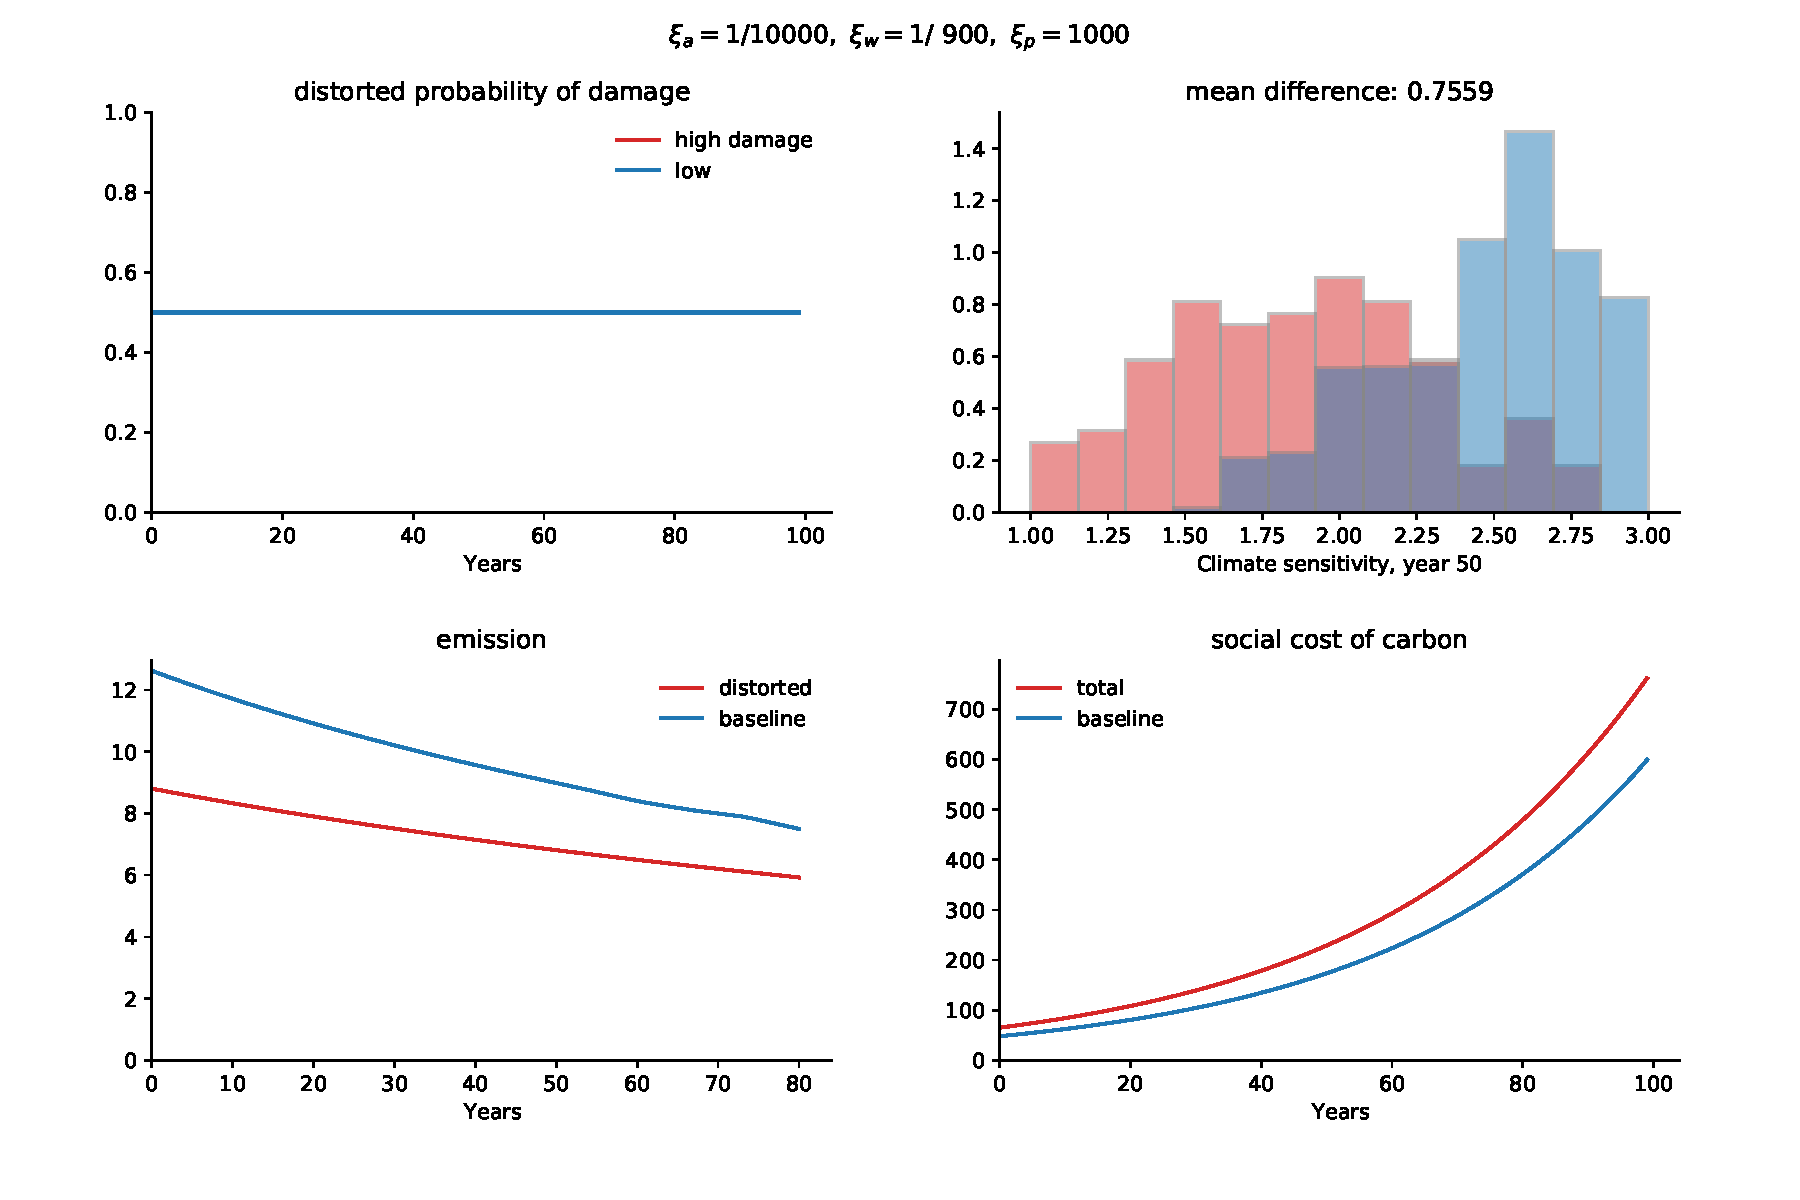
\includegraphics[width=\linewidth]{notebook/10_900_1000.pdf}
            \caption{\(\xi_p=1000\)}
            \label{fig:notebook/10_900_90}
        \end{figure}
        \newpage
    \item \(\xi_p= 90\xi_w\)
        \begin{figure}[H]
            \centering
            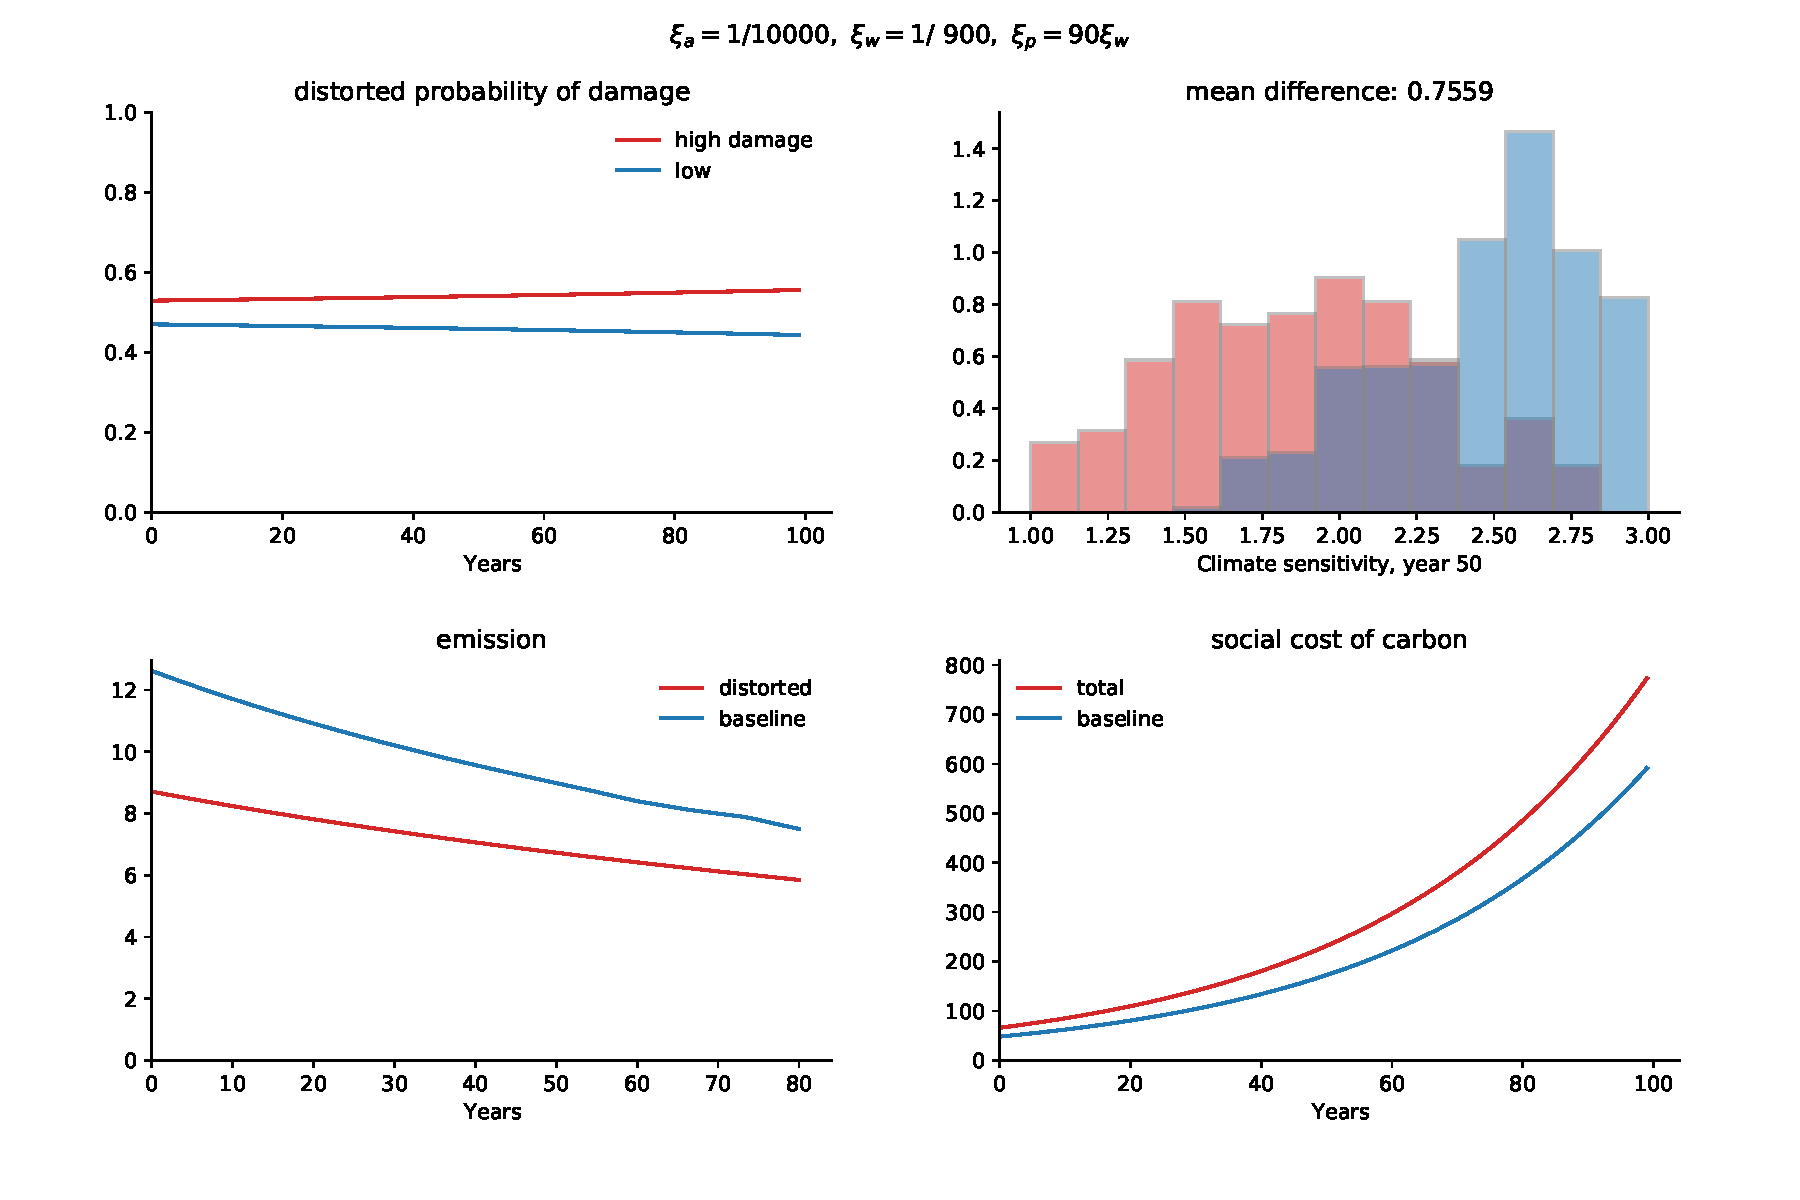
\includegraphics[width=\linewidth]{notebook/10_900_90.pdf}
            \caption{\(\xi_p=90\xi_w\)}
            \label{fig:notebook/10_900_90}
        \end{figure}
        \newpage
    \item \(\xi_p=45\xi_w\)
        \begin{figure}[H]
            \centering
            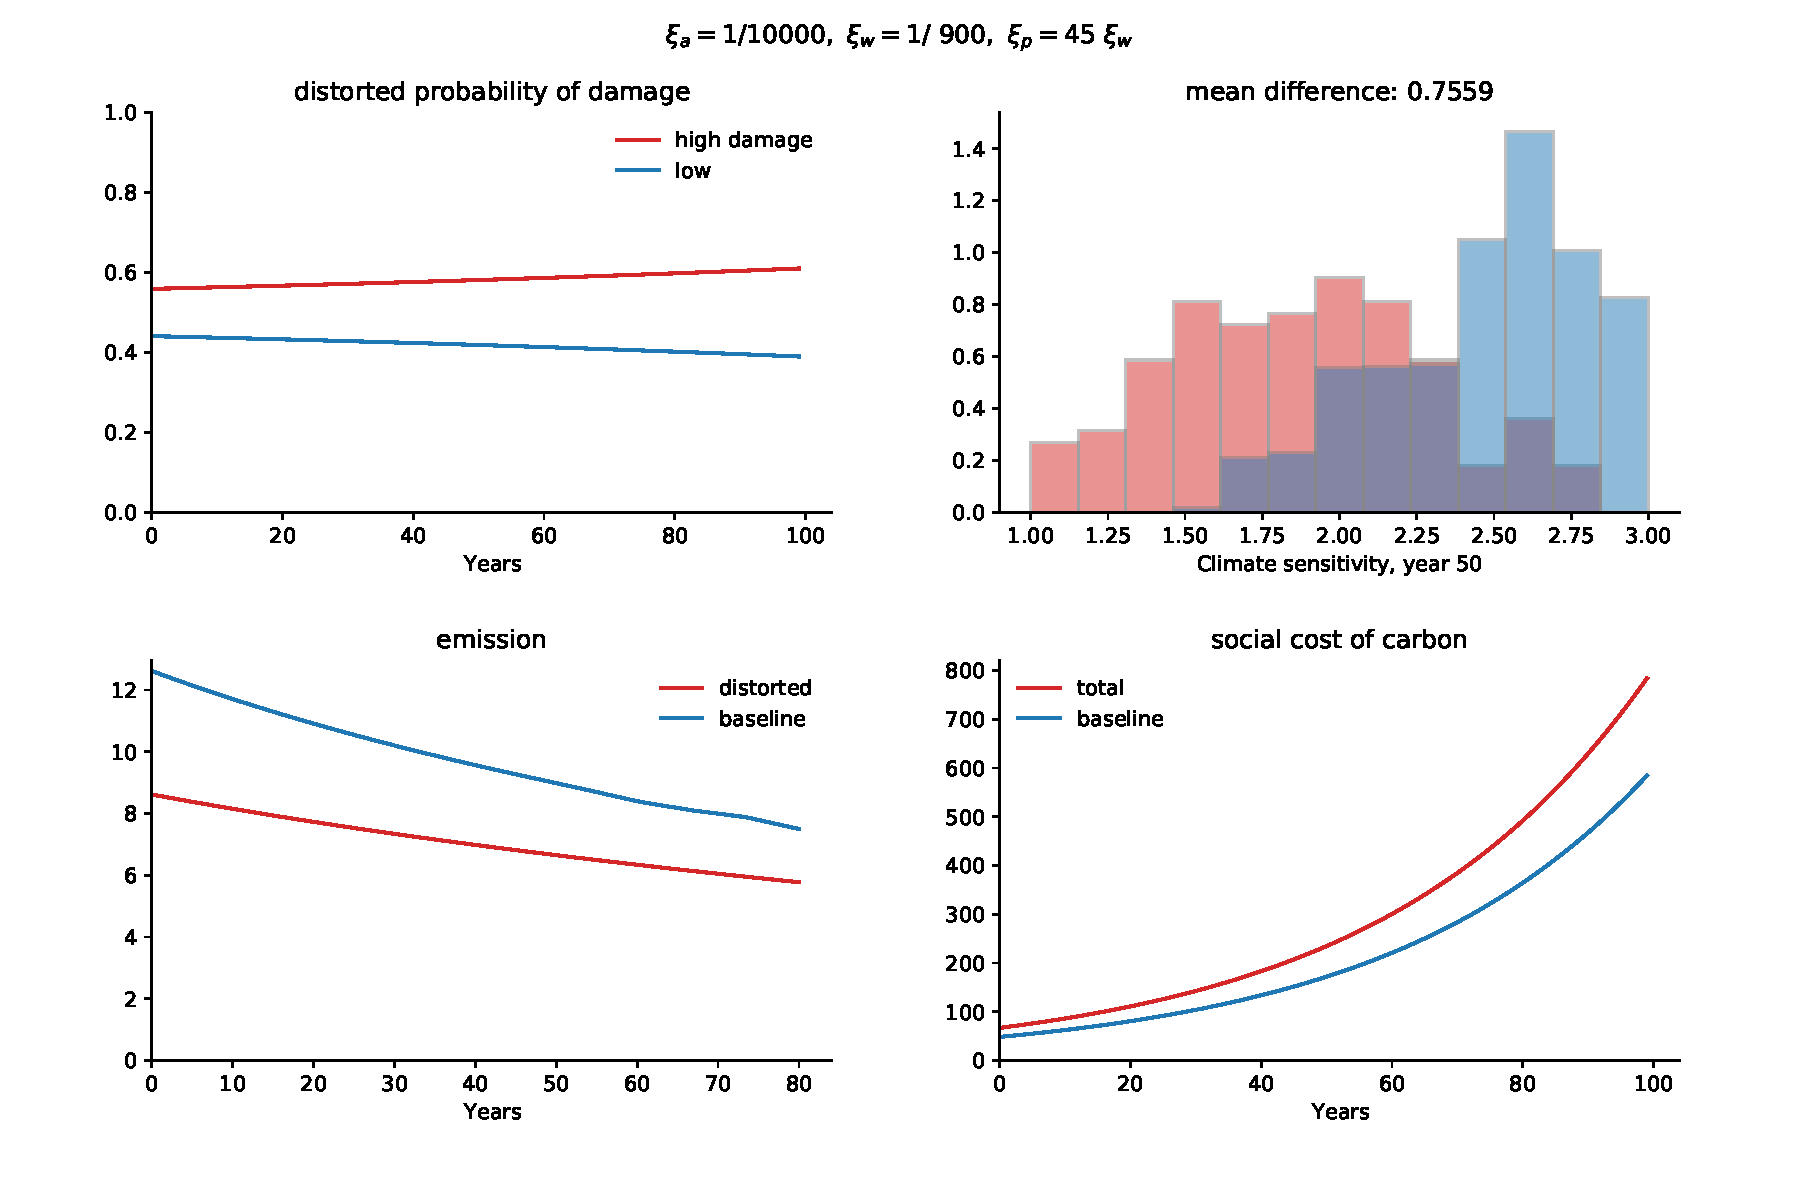
\includegraphics[width=\linewidth]{notebook/10_900_45.pdf}
            \caption{\(\xi_p=45\xi_w\)}
            \label{fig:notebook/10_900_45}
        \end{figure}
        \newpage
    \item \(\xi_p=\xi_w\)
        \begin{figure}[H]
            \centering
            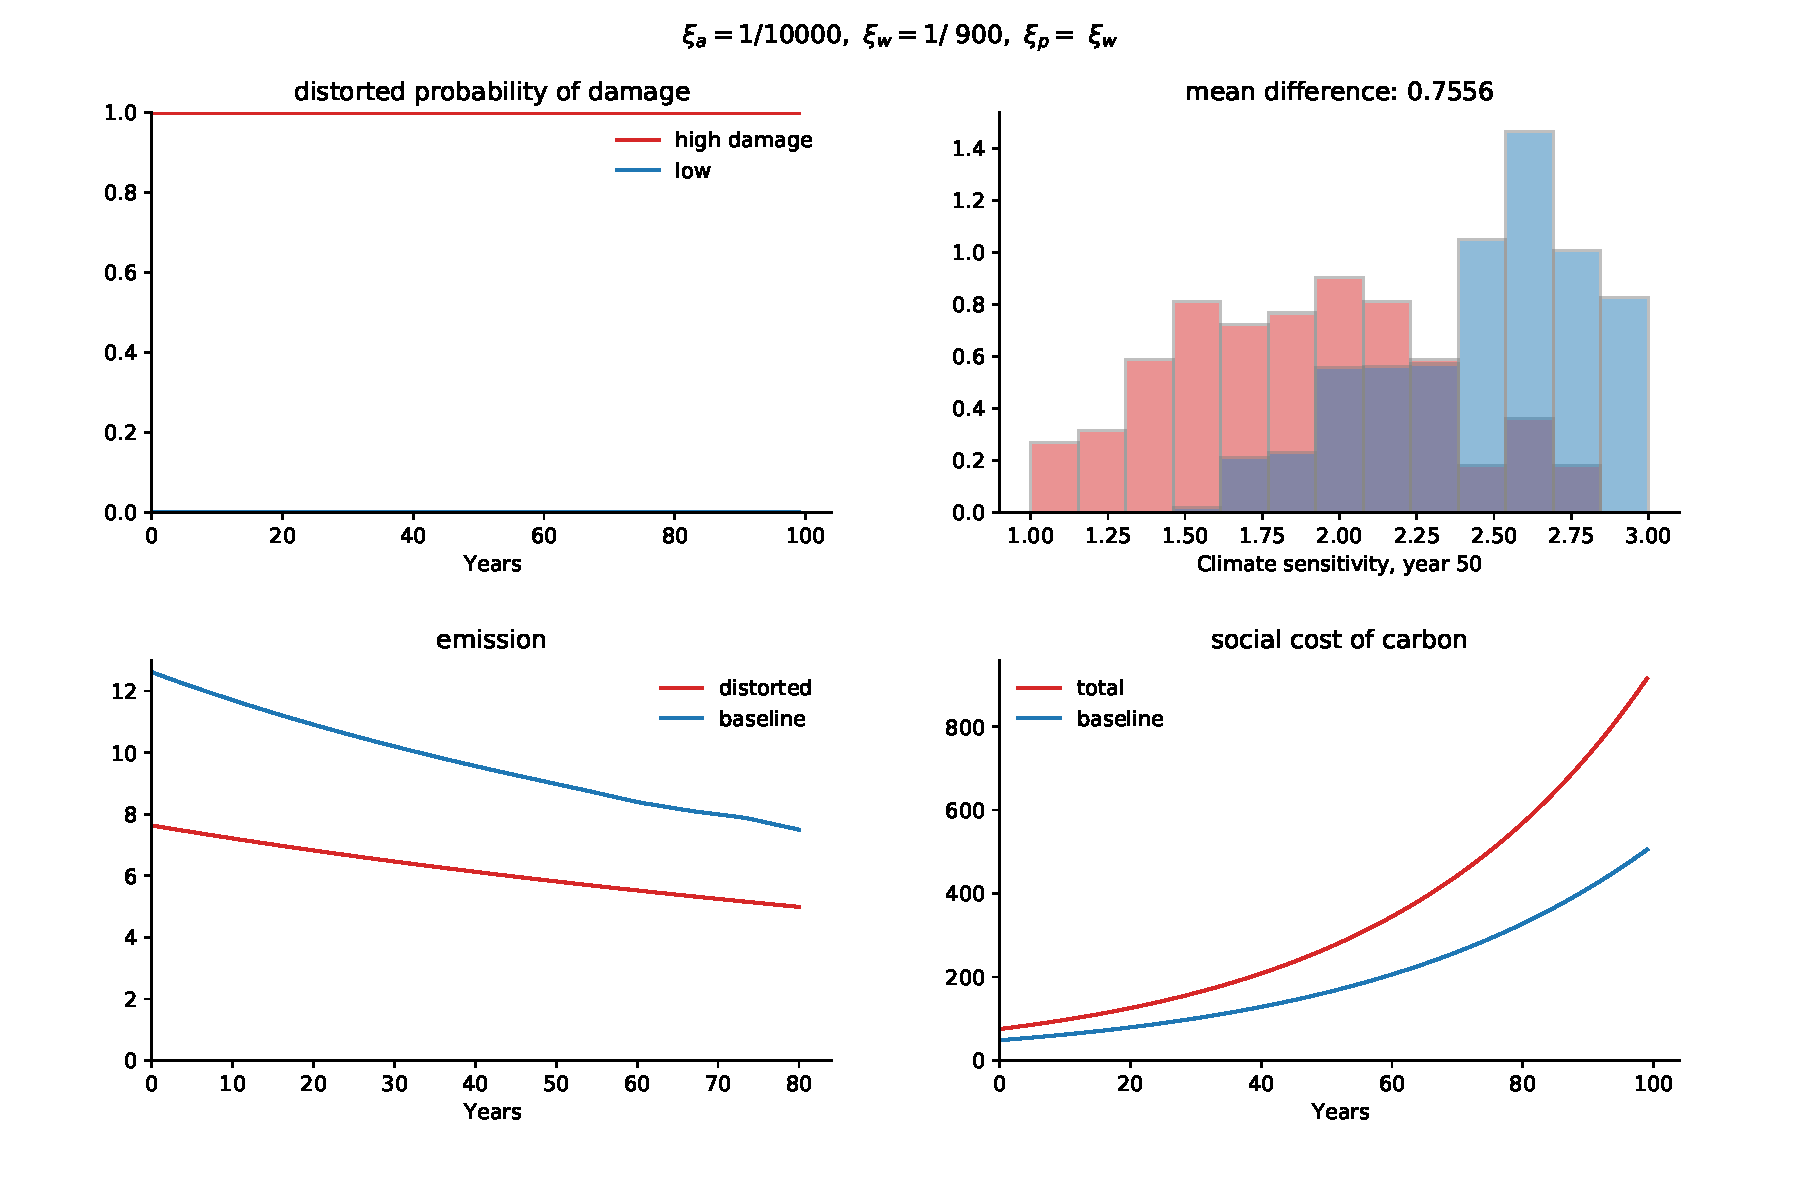
\includegraphics[width=\linewidth]{notebook/10_900_1.pdf}
            \caption{\(\xi_p=\xi_w\)}
            \label{fig:notebook/10_900_45}
        \end{figure}
\end{itemize}
\end{document}
